\documentclass[sigconf]{acmart}
\usepackage[utf8]{inputenc}
\usepackage{amsfonts,amsmath,amssymb,amsthm,amstext,latexsym}
\usepackage{subfig}
%\usepackage{mathdots}
\usepackage{url}
\usepackage{makecell}
\usepackage{multirow}
\usepackage{tikz}
\usepackage[textwidth=2cm]{todonotes}
\usetikzlibrary{calc}
\usetikzlibrary{arrows,shapes}
\usetikzlibrary{patterns,decorations}
\newtheorem{theorem}{Theorem}
%opening

%\newcommand\leo[1]{\textcolor{blue}{#1}}
%\newcommand\ldo[1]{\todo[fancyline, size=\tiny, backgroundcolor=cyan]{#1}{}}

%\newcommand\marc[1]{\textcolor{red}{#1}}


\newcommand\leo[1]{\textcolor{black}{#1}}
\newcommand\ldo[1]{\ignorespaces}



\pagestyle{plain}

\title{Approximating a Multi-Grid Solver}

\author{Valentin Le F\`{e}vre}
    \affiliation{\'{E}cole Normale Supérieure de Lyon}
     \email{valentin.le-fevre@ens-lyon.fr}

\author{Leonardo Bautista-Gomez}
    \affiliation{Barcelona Supercomputing Center (BSC)}
    \email{leonardo.bautista@bsc.es}

\author{Osman Unsal}
    \affiliation{Barcelona Supercomputing Center (BSC)}
    \email{osman.unsal@bsc.es}

\author{Marc Casas}
    \affiliation{Barcelona Supercomputing Center (BSC)}
    \email{marc.casas@bsc.es}

\begin{document}

\maketitle
\begin{abstract}

    Multi-grid methods are numerical algorithms used in parallel and
    distributed processing. The main idea of multi-grid solvers is to speedup
    the convergence of an iterative method by reducing the problem to a coarser
    grid a number of times. Multi-grid methods are widely exploited in many
    application domains, thus it is important to improve  their performance and
    energy efficiency. This paper aims to reach this objective based on the
    following observation: Given that the intermediary steps do not require
    full accuracy, it is possible to save time and energy by reducing precision
    during some steps while keeping the final result within the targeted
    accuracy.

    To achieve this goal, we first introduce a cycle shape different from
    the classic V-cycle used in multi-grid solvers.  Then, we propose to
    dynamically change the floating-point precision used during runtime
    according to the accuracy needed for each intermediary step. Our evaluation
    with the BoomerAMG multi-grid solver demonstrates that it is possible to
    trade temporary precision for time to completion without hurting the
    quality if the final result.  In particular, we are able to reach the same
    accuracy results as with full double-precision while gaining between 15\%
    and 30\% execution time improvement.

\end{abstract}

%% Section I
\section{Introduction}
\label{sec:intro}

Multi-Grid (MG) solvers are a class of linear methods~\cite{Hackbusch1991} that
emerged in the 80's to increase the convergence rate of more classical
iterative methods.  They became even more important with the advent of very
complex scientific applications~\cite{Ashby1996}, which required very powerful
linear solvers.  The usage of MG solvers has become a common practice in
today's parallel systems due to the good scalability properties this methods
display, which have been detailedly analyzed and modeled~\cite{Gahvari11}.
Also, MG solvers have been reported to display more robustness against silent
data corruptions than traditional iterative methods deployed over a single
grid~\cite{Casas12}, which also implies they behave well under reduced accuracy
scenarios.

Multi-Grid\ldo{Are we going to use MG or Multi-Grid? We should be consistent}
algorithms rely on a grid of evaluation points that discretize the
domain of a continuous differential equation.  Typically, MG schemes are
defined by coarsening a fine-grain grid until reaching a small set of
evaluation points where a direct method can be applied.
%This grid is represented using different granularity levels that are used to
%determine a solution on the inaccurate and coarse grids.
Solutions obtained on the inaccurate and coarse grids are used on the more
accurate and fine-grain levels to accelerate the process of obtaining the final
solution of the system.
%For example, if we want to solve an equation of the form: \[ -u^{''}(x)+au(x)
%= f(x),\quad 0<x<1, \quad u(0)=u(1)=0, \] where $a$ is some constant, $f$ a
%function and $u$ an unknown function, we can transform it into a discrete
%problem by selecting $N$ evaluation points $x_1,\dots,x_N$ and using taylor
%expansion to express the second derivative term $u^{''}(x_i)$ as a weighted
%sum of $u(x_j)$ for some values of $j$.  Then to define coarser grids, a
%simple way to do it is to divide the number of evaluation points and transform
%the original equation into another discrete problem (thus using evaluation
%points $x_1,x_3,\dots,x_N$).  Typically, multi-grid schemes are defined by
%coarsening a fine-grain grid until reaching a small enough set of evaluation
%points on which a direct solve would be fast.
Multi-grid solvers typically consist of three phases: The \textit{Relaxation},
\textit{Restriction} and \textit{Interpolation} phases.  The relaxation phase
applies a few steps of an iterative solver like Jacobi or Gauss-Seidel at a
certain coarseness level.  The restriction phase propagates the algorithmic
state to a coarser grid by means of linear transformations while the
interpolation phase maps the coarser estimate to the finer version and adjusts
the current solution with the new error.

One common way of orchestrating a Multi-Grid Solver execution is via a V-cycle,
where we first iterate on the finest grid, then the second finest grid and so
on until reaching the coarsest grid where a direct solve is used instead of an
iterative method as the problem size has become smaller.  Then we iterate again
on all the other grids in the reverse order to have a solution expressed with
the initial fineness of the grid.  Different parameters, such as the iterative
method used at each step or the fineness of the grid and the previously
mentioned cycle shape, affect the convergence rate of the algorithm.

%Typically, multi-grid schemes are defined by coarsening a fine-grain grid
%until reaching a small enough set of evaluation points on which a direct solve
%would be fast.  Multi-grid solvers then perform several steps of an iterative
%method like Jacobi~\cite{} or Gauss-Seidel~\cite{} switching between the
%different grids by interpolating or restricting the solution of the previous
%step.  More precisely, a multi-grid algorithm has a parameter which is the
%cycle shape.  The cycle shape determines in which order and on which
%coarsening of the grid an iterative method is used. The classical cycle shape
%is the V-cycle where we first iterate on the finest grid, then the second
%finest grid and so on until reaching the coarsest grid where a direct solve is
%used instead of an iterative method as the problem size has become smaller.
%Then we iterate again on all the other grids in the reverse order to have a
%solution expressed with the initial fineness of the grid.  Different
%parameters, such as the iterative method used at each step or the fineness of
%the grid and the previously mentioned cycle shape, affect the convergence rate
%of the algorithm. For example, using a grid with only a few evaluation points
%decreases the execution time but deteriorates the accuracy of the final
%result. In the other way, it is possible to increase the quality of the result
%by using a finer grid but at the cost of a performance degradation.

In this context, this paper investigates different trade-offs between accuracy
and execution time for MG algorithms. This paper focuses its effort on
one of the most popular parallel implementation of a multi-grid solver, the
BoomerAMG~\cite{boomerAMG}, implemented in the HYPRE
library~\cite{Falgout2002}.  This paper makes the following contributions
beyond the state-of-the-art:

\begin{itemize}

    \item We evaluate the impact of parameters of the solver such as the shape
        of cycles and the number of iterations.

    \item We propose a cycle configuration and show that it is equally or more
        efficient than the original algorithm.

    \item We \leo{evaluate the impact of different floating-point precisions on
        the time to completion while reaching full accuracy on the final
        result.}

    \item We propose an algorithm that dynamically adapts the precision of the
        MG algorithm variables to increase performance and efficiency.

    \item We \leo{perform a large evaluation and demonstrate the we can reduce by
        15\% the execution time needed to reach the same quality result as the
        original double-precision algorithm and up to 30\% for smaller
        accuracies.}

\end{itemize}


\leo{The reminder of this paper is organized as follows: Section~\ref{sec:algo}
introduces the MG algorithm briefly. Section~\ref{sec:pruning} investigates the
impact of different parameters on the time to completion.
Section~\ref{sec:precision} explores precision-performance trade-offs.
Section~\ref{sec:related} discuss other related works and
Section~\ref{sec:conclusions} concludes this paper.}



%% Section II
\section{Motivation and Background}
\label{sec:motivation}

In high performance computing (HPC), maximizing performance is the main
objective. However, in order to reach extreme scale computing, it is necessary
to also improve the energy efficiency of current applications and algorithms.
This section explains why approximate computing is potential solution and why
MG solvers are a good candidate for this type of optimizations.

\subsection{Approximate Computing}
\label{sec:approx}

%\leo{A very brief introduction to approximate computing.. }
%\marc{

Approximate computing categorizes a wide set of techniques aimed at trading off computation's quality with cost.
It is based on the intuition that operating at peak level accuracy may produce significant resource waste without adding any valuable information to the numerical data.
The increasing restrictions that parallel architectures are suffering in terms of power and circuitry area have made the approximate computing field an appealing and cost-effective approach that can be potentially applied to a wide range of application domains like data analytics, scientific computing, multimedia or signal
processing~\cite{Mittal2016}.
Indeed, recent approaches demonstrate how up to 50x enery savings can be achieved when applying approximate computations to the k-means clustering algorithm while only losing 5\% classificatin accuracy~\cite{Chippa2013}.
Also, an approximate approach based on neural networks can speedup an inverse kinematics application by more than 20x by allowing a final application error of just 5\%~\cite{Grigorian2015}.

Despite its potential, approximate computing must be applied in an extremely careful way.
For example, reducing the accuracy of control flow instructions or memory addresses computations may cause segmentation faults.
Also, applying approximate techniques to floating point computations can potentially bring wrong results or cause iterative algorithms to stall if they are blindly applied.
The success of approximate approaches requires them to be judicisouly applied to the most low-accuracy tolerant phases of numerical algorithms.
In this paper we apply approximate computing approaches to the MG solver in several different ways.
Some of them reduce the amount of computations of certain routines while keep the accuracy of each computation, like reducing on the number of relaxation iterations (Section~\ref{sec:pruning}).
Other approaches keep the number of computations but reduce their accuracy, like using floating point representations with less bits devoted to store the mantissa (Section~\ref{sec:precision}).

 


%}

\begin{figure}[hbt]
 \resizebox{\linewidth}{!}{
    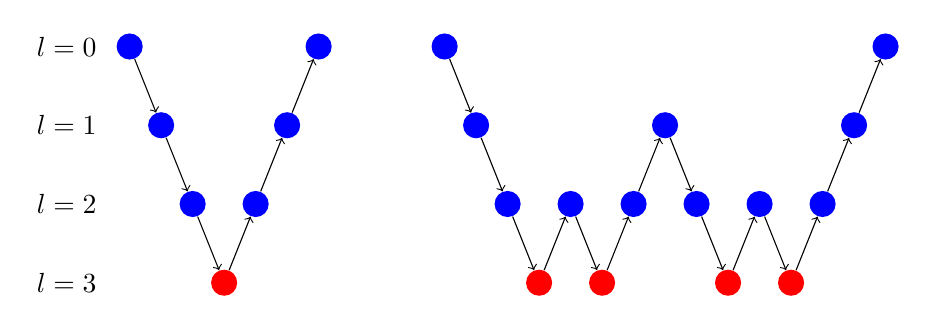
\begin{tikzpicture}

 \begin{scope}[xscale=2/5]

  \node (sh) at (-5,3) { $l=0$ };
  \node (shh) at (-5,2) { $l=1$ };
  \node (shhh) at (-5,1) { $l=2$ };
  \node (shhhh) at (-5,0) { $l=3$};

  %\node (title) at (0,5) { V-cycle k=1};
  %\node (title2) at (14,5) {W-cycle k=2};

    \node[circle,fill=blue] (a) at (-3,3) { };
    \node[circle,fill=blue] (b) at (-2,2) {};
    \node[circle,fill=blue] (c) at (-1,1) {};
    \node[circle,fill=red] (d) at (0,0) {};
    \node[circle,fill=blue] (e) at (1,1) {};
    \node[circle,fill=blue] (f) at (2,2) {};
    \node[circle,fill=blue] (g) at (3,3) {};

    \draw[->] (a) -- (b);
    \draw[->] (b) -- (c);
    \draw[->] (c) -- (d);
    \draw[->] (d) -- (e);
    \draw[->] (e) -- (f);
    \draw[->] (f) -- (g);

    \node[circle,fill=blue] (aa) at (7,3) { };
    \node[circle,fill=blue] (ab) at (8,2) {};
    \node[circle,fill=blue] (ac) at (9,1) {};
    \node[circle,fill=red] (ad) at (10,0) {};
    \node[circle,fill=blue] (ae) at (11,1) {};
    \node[circle,fill=red] (af) at (12,0) {};
    \node[circle,fill=blue] (ag) at (13,1) {};
    \node[circle,fill=blue] (ah) at (14,2) {};
    \node[circle,fill=blue] (ai) at (15,1) {};
    \node[circle,fill=red] (aj) at (16,0) {};
    \node[circle,fill=blue] (ak) at (17,1) {};
    \node[circle,fill=red] (al) at (18,0) {};
    \node[circle,fill=blue] (am) at (19,1) {};
    \node[circle,fill=blue] (an) at (20,2) {};
    \node[circle,fill=blue] (ao) at (21,3) {};

    \draw[->] (aa) -- (ab);
    \draw[->] (ab) -- (ac);
    \draw[->] (ac) -- (ad);
    \draw[->] (ad) -- (ae);
    \draw[->] (ae) -- (af);
    \draw[->] (af) -- (ag);
    \draw[->] (ag) -- (ah);
    \draw[->] (ah) -- (ai);
    \draw[->] (ai) -- (aj);
    \draw[->] (aj) -- (ak);
    \draw[->] (ak) -- (al);
    \draw[->] (al) -- (am);
    \draw[->] (am) -- (an);
    \draw[->] (an) -- (ao);

 \end{scope}

\end{tikzpicture}


 }
 \caption{V-cycle and W-cycle on 4-level grid.}
 \label{fig.cycles}
\end{figure}

\subsection{Multi-Grid Algorithm}
\label{sec:algo}

MG's cycles start and end on the finest grained grid and are defined by the
order in which its different coarseness levels are applied.  The simplest cycle
is the V-cycle, already described in Section~\ref{sec:intro}, where a few
iterations of an iterative method (the \textit{Relaxation} step) is performed
at each level from the finest to the coarsest level and then in the reverse
order.  Another common approach is the W-cycle scheme where the coarsest grid
level is reached several times before going back to the finest grid level.  It is
possible to generalize the notion of cycle to a $k$-cycle (where a V-cycle is a
$1$-cycle and a W-cycle is a $2$-cycle).  Figure~\ref{fig.cycles} shows a
representation of the V- and the W-cyles with 4 levels where we can see how the
W-scheme goes back and forth the coarsest level 4 times before reaching again
the finest level of the grid.  The cycles are executed multiple times
iteratively until the error is lower or equal to a certain \emph{tolerance}
(i.e., the expected accuracy) or until the maximum number of cycles is reached.

%\subsection{Definitions}

%\begin{itemize}
% \item A system of equations is represented by the following equation: $Ax=b$, where $A \in \mathcal{M}(\mathbb{R})^{n\times n}$ and $b \in \mathcal{\mathbb{R}}^n$ are given and
% $x \in \mathbb{R}^n$ is the unknown. The \emph{exact} solution of this system will be denoted by $\widetilde{x}$.
% \item A level is an integer between $1$ and $L$. Level $1$ will be called the finest level, and level $L$ will be called the coarsest level.
%  \item The restriction of $A$ (or $b$ or $x$) to level $l$ will be denoted by $A^l$ (or $b^l$ or $x^l$). We have $A^1 = A$ (and $b^1=b,x^1=x$).
%  \item We define a set of $L-1$ restriction matrices $R_1,\dots,R_{L-1}$ such that $R_l b^l = b^{l+1}$. We also define some prolongation matrices $P_1,\dots,P_{L-1}$ such that $P_{l}b^{l+1} = b^l$.
%  In other words, we have $P_l = {R_l}^{-1}$ (left inverse) and we build the $A^l$ matrices as follows: $A^{l+1} = R_l A^l P_l$.
%  \item We denote by $e^l$ the error at level $l$, that is the vector such that $x^l + e^l = \widetilde{x^l}$, that is to say $\widetilde{x^l}-x^l$.
%  We also define the residual at level $l$, $r^l = b^l - A^lx^l$. As $b^l = A^l\widetilde{x^l}$, we can also write $r^l = A^le^l$.
%  \item We derive the relative residual norm at any step $i$ in the algorithm
%  by the norm of the residual at this step, $||b^l - A^lx^l_i||$, divided by the norm of the initial residual, $|| b^l - A^lx^l_0||$.\\ We also define the notion of \emph{tolerance}
%  as an real value between 0 and 1, which is a threshold for stopping an algorithm. In multi-grid algorithms, this threshold will be on the residual norm.
%  \item We call relaxation a step of an iterative method for solving linear systems (such as Jacobi, Gauss-Sneidel, \dots). Formally, for a vector $x \in \mathbb{R}^n$, it represents the computation of
%  $x \leftarrow Mx + c$ where $M \in \mathcal{M}(\mathbb{R})^{n\times n}$ and $c \in \mathcal{\mathbb{R}}^n$ are defined depending on the method used.
% \end{itemize}

%\subsection{The V-cycle}

%  The goal of the algorithm is to improve the efficiency of iterative methods.
%  Indeed, the choice of the starting vector $x$ on which to apply relaxations
%  has consequences on the convergence time of the solver, and depending on the
%  system to solve, the factor of convergence (related to the matrix $M$) can
%  be close to 1.\\ Here the idea is to do some relaxations and then correct
%  the value of $x$ by adding to it the corresponding error term. However, this
%  error term cannot be computed easily (otherwise, solving the problem would
%  be done by computing the error term and adding it to $x$). Multi-grid
%  solvers instead use recursion to compute the error term. The stopping
%  parameter for the recursion will be determined by decreasing the sizes of
%  vectors and matrices (thus loosing some accuracy but saving time).
%  Formally, we can sum up the algorithm as follows:


%  MG$(l,x,f,\alpha_1,\alpha_2)$:
%  \begin{itemize}
%    \item If $l = L$, return $x = {A^L}^{-1} f$ (exact solve);
%    \item Else:
%    \begin{enumerate}
%      \item Relax $x$ $\alpha_1$ times using an iterative method (matrix $A^l$, right hand side $f$);
%      \item $r \leftarrow R_l ( f - Ax )$;
%      \item $y \leftarrow 0$:
%      \item MG$(l+1,y,r,\alpha_1,\alpha_2)$;
%      \item $e \leftarrow P_{l} y$;
%      \item $x \leftarrow x+e$;
%      \item Relax $x$ $\alpha_2$ times using an iterative method (matrix $A^l$, right hand side $f$);
%   \end{enumerate}
%  \end{itemize}
%  The algorithm is then executed by setting $x^l \leftarrow 0$ and then executing MG$(1,x^l,b^l,\alpha_1,\alpha_2)$.
%
%  Then several ways of modifying the algorithm appear:
%  \begin{itemize}
%   \item Which iterative method to use?
%   \item Do we want only one recursive call at each level or more?
%   \item How many times do we need to apply the algorithm?
%   \item How to determine good $\alpha_1$ and $\alpha_2$ parameters?
%   \item How many levels should be defined?
%  \end{itemize}
%
%  In all what follows the iterative method chosen is an hybrid
%  Jacobi/Gauss-Seidel method. The number of levels used will not be studied.






%% Section III

\subsection{Comparing Different Kinds of Cycles}

%  A level is an integer between $1$ and $L$. Level $1$ will be called the finest level, and level $L$ will be called the coarsest level. In the multi-grid algorithm, we
%  consider computations at every different level in a determined order. 
In this Section we compare different types of cycles and study how the number of \textit{Relaxation} steps influence MG's convergence.
MG's cycles start and end on the finest grained grid and are defined by the order in which its different coarseness levels are applied.
The simplest cycle is the V-cycle, already described in Section~\ref{sec:intro}, where a few iterations
  of an iterative method (the \textit{Relaxation} step) is performed at each level from the finest to the coarsest level and then in the reverse order. 
Another common approach is the W-cycle scheme where the coarsest grid level is reached twice before going back to the finest grid level.
It is possible to generalize the notion of cycle to a $k$-cycle (where a V-cycle is a $1$-cycle and a W-cycle is a $2$-cycle).
Figure~\ref{fig.cycles} shows a representation of the V- and the W-cyles with 4 levels where we can see how the W-scheme goes back and forth the coarsest level 4 times before reaching again the finest level of the grid.

%In this context, the MG algorithm makes use of many different input parameters 
% such as the iterative method used, the type of cycle and its number of repetitions, the number of \textit{Relaxation} at each level or the number of different levels to define.
%In this subsection we focus on comparing different types of cycles and study how the number of \textit{Relaxation} steps influence the convergence of the algorithm.
  
%We consider 2 types of cycles: the V-cycle and the W-cycle. 
%The main difference between them is that in the W-cycle the recursive call
%to a coarser grid is made twice instead of one before going back to a finer level. 
%We call these cycles V-cycle and W-cycle because of how we can draw them if we represent each time relaxations are done
%  at a level by a point (see Figure~\ref{fig.cycles}). 
%Figure~\ref{fig.cycles} shows a representation of the V- and the W-cyles.
%It is possible to define other types of cycles by adding more and more repeats of these steps (do $k$ times those steps) to generalize
%  the notion of cycle to a $k$-cycle (where a V-cycle is a $1$-cycle and a W-cycle is a $2$-cycle).
  
 \begin{figure}
 \resizebox{\linewidth}{!}{
 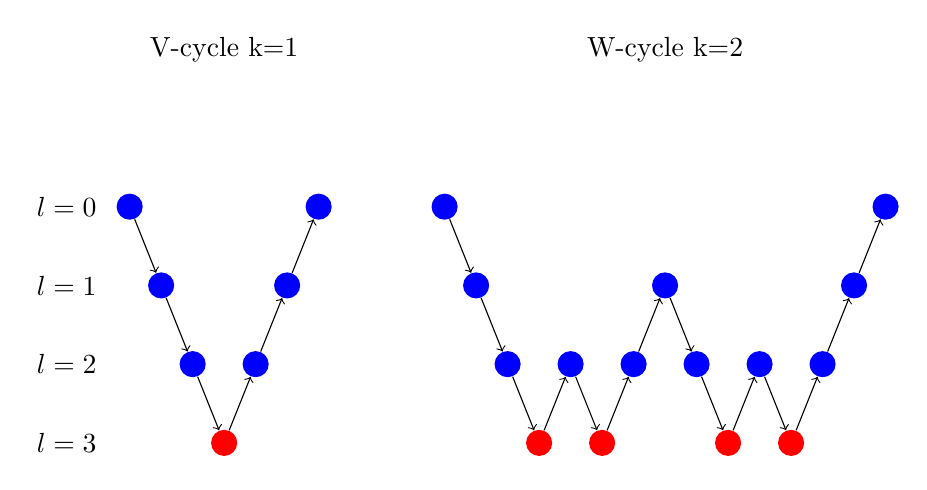
\begin{tikzpicture}
  
\begin{scope}[xscale=2/5]

  \node (sh) at (-5,3) { $l=0$ };
  \node (shh) at (-5,2) { $l=1$ };
  \node (shhh) at (-5,1) { $l=2$ };
  \node (shhhh) at (-5,0) { $l=3$};
  
  \node (title) at (0,5) { V-cycle k=1};
  \node (title2) at (14,5) {W-cycle k=2};

    \node[circle,fill=blue] (a) at (-3,3) { };
    \node[circle,fill=blue] (b) at (-2,2) {};
    \node[circle,fill=blue] (c) at (-1,1) {};
    \node[circle,fill=red] (d) at (0,0) {};
    \node[circle,fill=blue] (e) at (1,1) {};
    \node[circle,fill=blue] (f) at (2,2) {};
    \node[circle,fill=blue] (g) at (3,3) {};
    
    \draw[->] (a) -- (b);
    \draw[->] (b) -- (c);
    \draw[->] (c) -- (d);
    \draw[->] (d) -- (e);
    \draw[->] (e) -- (f);
    \draw[->] (f) -- (g);
    
    \node[circle,fill=blue] (aa) at (7,3) { };
    \node[circle,fill=blue] (ab) at (8,2) {};
    \node[circle,fill=blue] (ac) at (9,1) {};
    \node[circle,fill=red] (ad) at (10,0) {};
    \node[circle,fill=blue] (ae) at (11,1) {};
    \node[circle,fill=red] (af) at (12,0) {};
    \node[circle,fill=blue] (ag) at (13,1) {};
    \node[circle,fill=blue] (ah) at (14,2) {};
    \node[circle,fill=blue] (ai) at (15,1) {};
    \node[circle,fill=red] (aj) at (16,0) {};
    \node[circle,fill=blue] (ak) at (17,1) {};
    \node[circle,fill=red] (al) at (18,0) {};
    \node[circle,fill=blue] (am) at (19,1) {};
    \node[circle,fill=blue] (an) at (20,2) {};
    \node[circle,fill=blue] (ao) at (21,3) {};
    
    \draw[->] (aa) -- (ab);
    \draw[->] (ab) -- (ac);
    \draw[->] (ac) -- (ad);
    \draw[->] (ad) -- (ae);
    \draw[->] (ae) -- (af);
    \draw[->] (af) -- (ag);
    \draw[->] (ag) -- (ah);
    \draw[->] (ah) -- (ai);
    \draw[->] (ai) -- (aj);
    \draw[->] (aj) -- (ak);
    \draw[->] (ak) -- (al);
    \draw[->] (al) -- (am);
    \draw[->] (am) -- (an);
    \draw[->] (an) -- (ao);
    \end{scope}
    
 \end{tikzpicture}}
 \caption{V-cycle and W-cycle on 4-level grid.}
 \label{fig.cycles}
\end{figure}

\begin{table}

\begin{center}
 \begin{tabular}{|c|c|c|c|c|c|c|c|c|}
   \hline
   Type of cycle & V & V & V & V & W & W & W & W \\
   \hline
   $\alpha$ & 1 & 2 & 3 & 10 & 1 & 2 & 3 & 10 \\
   \hline
 \end{tabular}
\end{center}
 \caption{8 strategies.}
 \label{table.strat1}

\end{table}


\begin{figure*}
  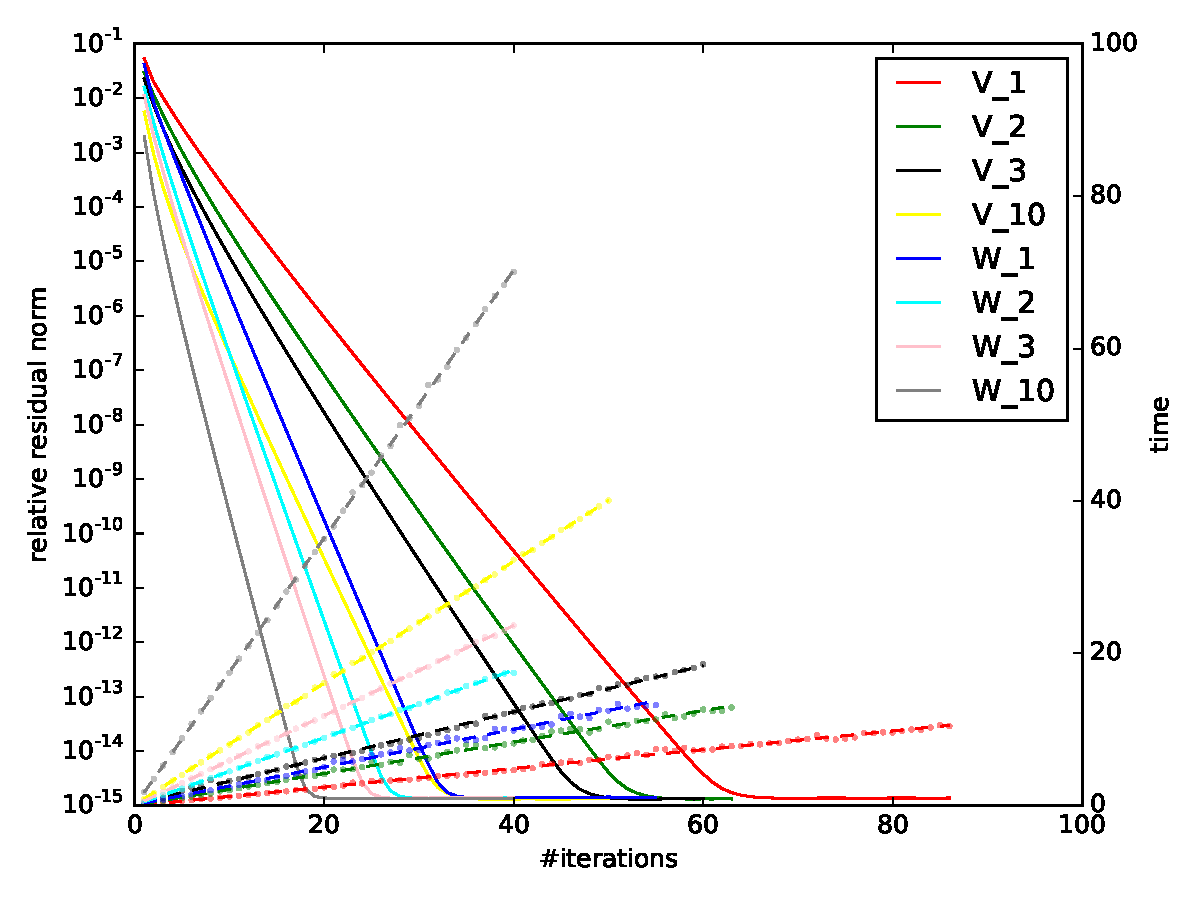
\includegraphics[width=0.49\linewidth]{figs/convergence_1.pdf}
  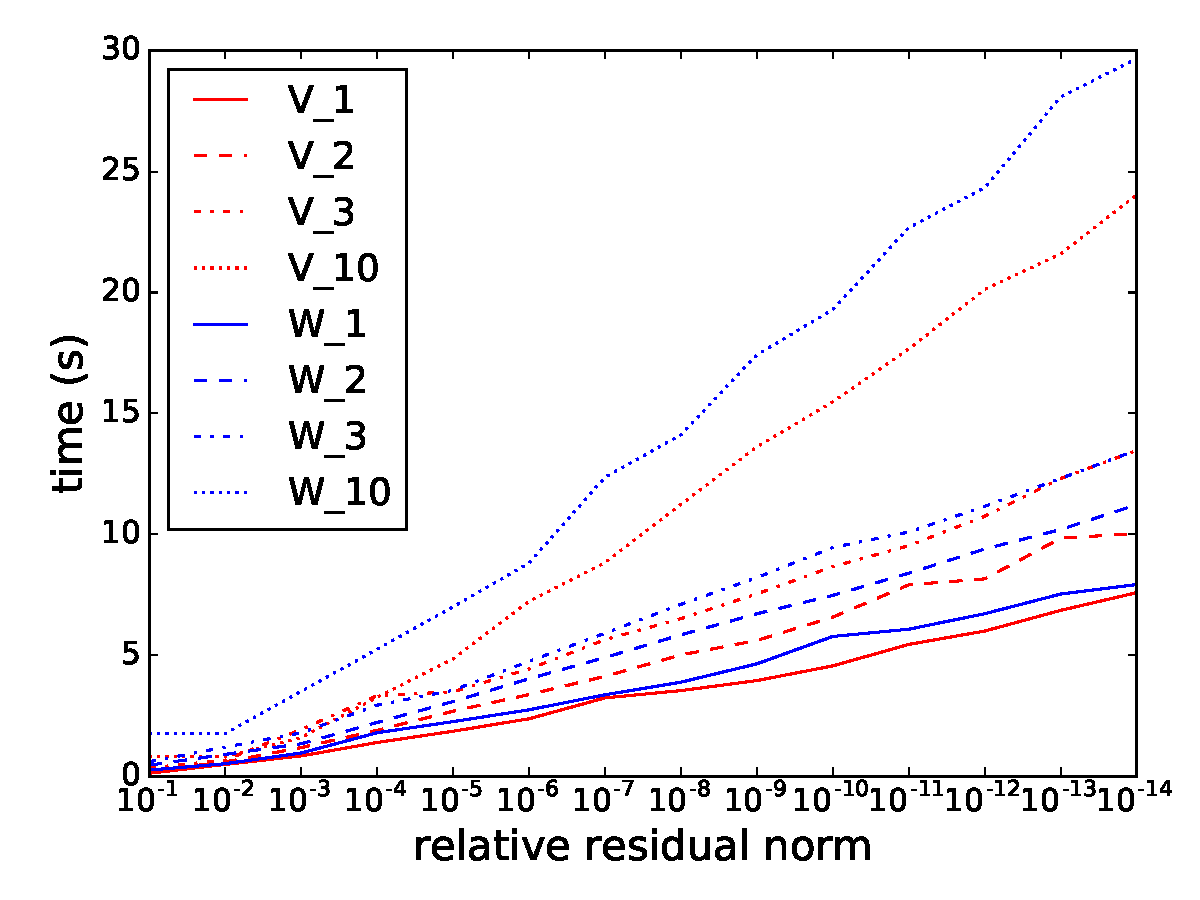
\includegraphics[width=0.49\linewidth]{figs/time_convergence.pdf}
  \caption{Execution time and final residual norm of the 8 strategies per iteration (left) and convergence time as a function of the tolerance (right).}
  \label{fig.first_tests}
\end{figure*}


The MG algorithm makes use of many different input parameters that have an impact on its success. 
% such as the iterative method used, the type of cycle and its number of repetitions, the number of \textit{Relaxation} steps per level or the number of different levels to define.
In our context, we define a strategy as a combination of values of the most relevant parameters: The type of cycle (V or W), the number of relaxation steps $\alpha$, and the total number of coarseness levels of the grid. 
%The default implementation of BomerAMG does not allow to have different values
%for $\alpha_1,\alpha_2,\dots$ so we set them all to this value $\alpha$. 
We consider a total of 8 different strategies represented in Table~\ref{table.strat1} where we consider V- and W-cycles and we perform 1, 2, 3 and 10 relaxation steps for eack kind of cycles, having a total of 8 configurations. 
The number of different coarseness levels of the grid is 8.
To compare the different strategies we consider an input matrix of size $512000 \times 512000$, 
and a maximum number of cycles from 1 to 100.
The algorithm's tolerance is set to $0$ to always reach the maximum number of cycles (1 to 100 depending on the experiments).
We measure for each experiment the final relative residual norm and the execution time. 
Each experiment is run 10 times to have an accurate average execution time.

The results are presented on Figure~\ref{fig.first_tests}.
The left figure shows how the accuracy evolve with the number of cycles performed (plain lines) while also showing the total execution time (dashed lines). The right figure expresses the cost of reaching
a given accuracy (left of the x-axis is a small tolerance i.e. correspond to accurate results while the right of the x-axis represent inaccurate (but fast) results).
What we can observe is that, as expected, increasing the number of relaxation steps or complexifying the cycle increases the overall time to do one cycle. However, it converges in less iterations.
We see on the right figure that actually, for a given precision, the simple V-cycle with only 1 relaxation at each step is the fastest way to reach it, followed closely by the W-cycle with $\alpha=1$.\\
The conclusion is that relaxation steps seem to be too costly for the accuracy they grant. It is better to increase the complexity of the cycle or do more cycles, thus more moves in the grid, than doing more relaxation steps. This at least proves
that multi-grid is a good alternative to classic iterative methods.

\subsection{\leo{Cycle Complexity Breakdown}}

Given the previous results, we embarked to investigate how to improve the
efficiency of the simple V-cycle with 1 relaxation step. The first step is to
breakdown the time spent in the different parts of a cycle. Note that all the
matrices for each level are computed in a setup phase and it is not necessary
to analyze that setup time. We only focus on measuring the following two
computations: (i) the time spent doing a relaxation at each level and (ii) the
time spent computing the next linear system. The latter (i.e., computing the
next linear system) can be divided in two options: \emph{going down} by
restricting the solution to a coarser grid, which corresponds to a sparse
matrix-vector computation; and \emph{going up} by interpolating the error term
which also corresponds to another sparse matrix-vector computation.

\begin{table}[htb]
 \resizebox{\linewidth}{!}{
 \begin{tabular}{|c|c|c|c|c|c|c|}
  \hline
  Level & \makecell{Matrix \\ size} & \makecell{Non-zero \\ elements} & \makecell{Relax \\ (down)} & \makecell{Relax \\ (up)} & \makecell{MatVec \\ (down)} & \makecell{MatVec \\ (up)} \\
  \hline
  1 & 512,000 & 4,042,520 & 20 ms & 20 ms & 15 ms & -\\
  \hline
  2 & 256,000 & 6,475,239 & 20 ms & 25 ms & 12 ms & 4 ms\\
  \hline
  3 & 58,893 & 2,000,513 & 8 ms & 8 ms & 3 ms & 2 ms\\
  \hline
  4 & 14,285 & 788,509 & 2 ms & 2 ms & 1 ms & 0.7 ms\\
  \hline
  5 & 4,238 & 386,333 & 1 ms & 1 ms & 0.5 ms & 0.2 ms\\
  \hline
  6 & 609 & 53,493 & $< 0.1$ ms & $< 0.1$ ms & $< 0.1$ ms & $< 0.1$ ms\\
  \hline
  7 & 69 & 2,873 & $< 0.1$ ms & $< 0.1$ ms & $< 0.1$ ms & $< 0.1$ ms\\
  \hline
  8 & 2 & 4 & $< 0.1$ ms & - & - & $< 0.1$ ms\\
  \hline
 \end{tabular}
 }
 \caption{Time breakdown of a V-cycle with $\alpha=1$.}
 \label{table.measures}
\end{table}

To study the internal time breakdown of a V-cycle we chose as problem an
unstructured domain with some anisotropy (denoted as Unstructured-Anisotropy)
of size 512,000 with a 8-level grid. The results of this evaluations are
depicted in Table~\ref{table.measures}, along with information on the matrix
used at the corresponding level, such as matrix size and the number of non-zero
elements.  Our first observation is that there is a direct correlation between
the time spent on relaxations at each given level and the number of non-zero
entries in the input matrix. Most importantly, in these results we observe that
relaxations represent $\approx66\%$ of the total cost of a V-cycle, while the
matrix-vector multiplications are only $\approx30\%$. In addition, we notice
that the two first levels are the most expensive ones.  It is important to
highlight that in the experiments depicted in Figure~\ref{fig.first_tests},
although different number of relaxations were evaluated, all levels executed
the \emph{same} number of relaxations.

\subsection{\leo{Level-Dependent Relaxation Tuning}}

Based on this information, we propose to reduce the execution time of a V-cycle
by tuning the number of relaxations differently for each level. More precisely
we propose the following two ideas: (i) to add more relaxations in the last
levels because their cost is negligible and they could potentially reduce the
time to convergence or (ii) to remove some relaxations in the first levels to
reduce the computational cost, and see how that affects convergence. We
translate these ideas into the four following strategies (based on a 8-level
grid):

\begin{itemize}
    \item \emph{Fast } : no relaxations at level 2.
    \item \emph{Fast2} : 10 relaxations at level 6.
    \item \emph{Fast3} :  2 relaxations at levels 6 and 4.
    \item \emph{Fast4} : no relaxations at level 3.
\end{itemize}

\begin{figure*}
    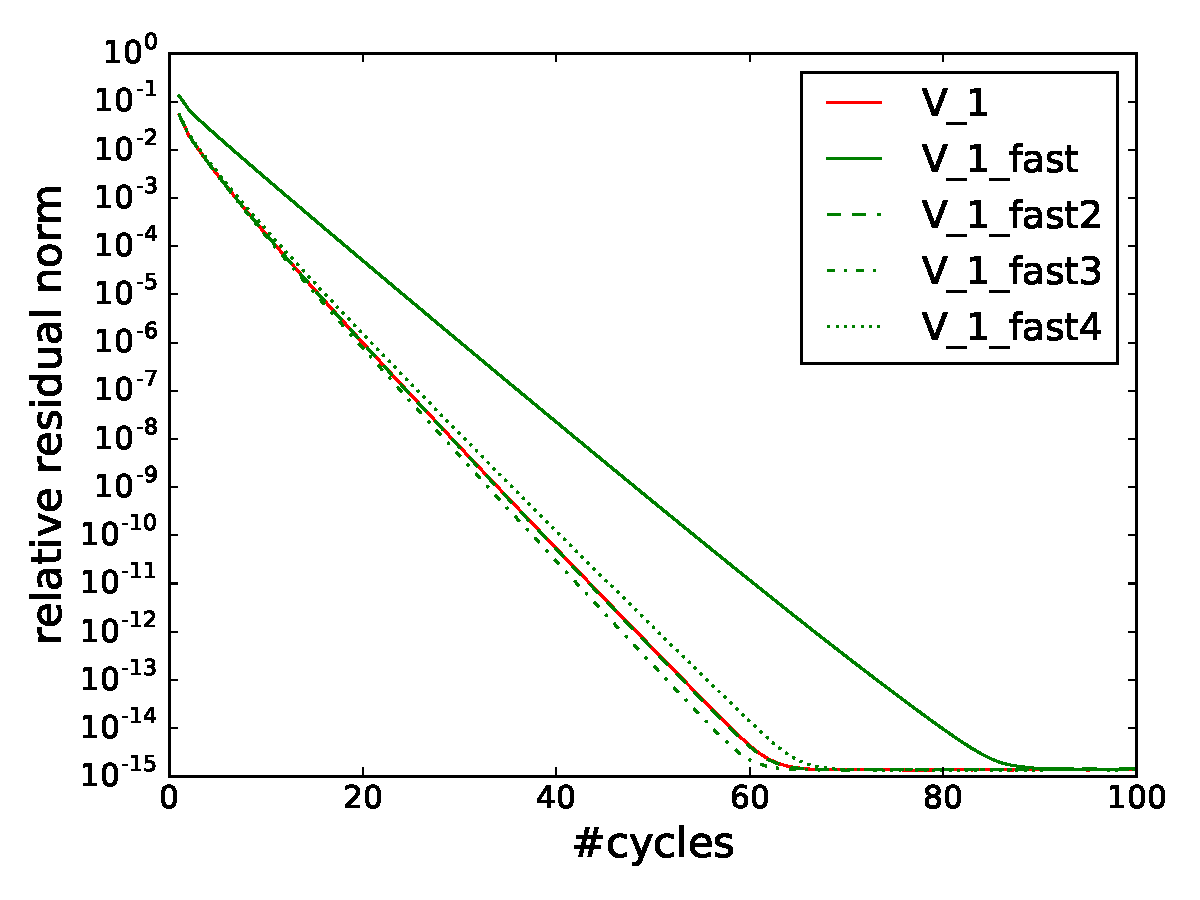
\includegraphics[width=0.33\linewidth]{figs/convergence_fast_norm.pdf}
    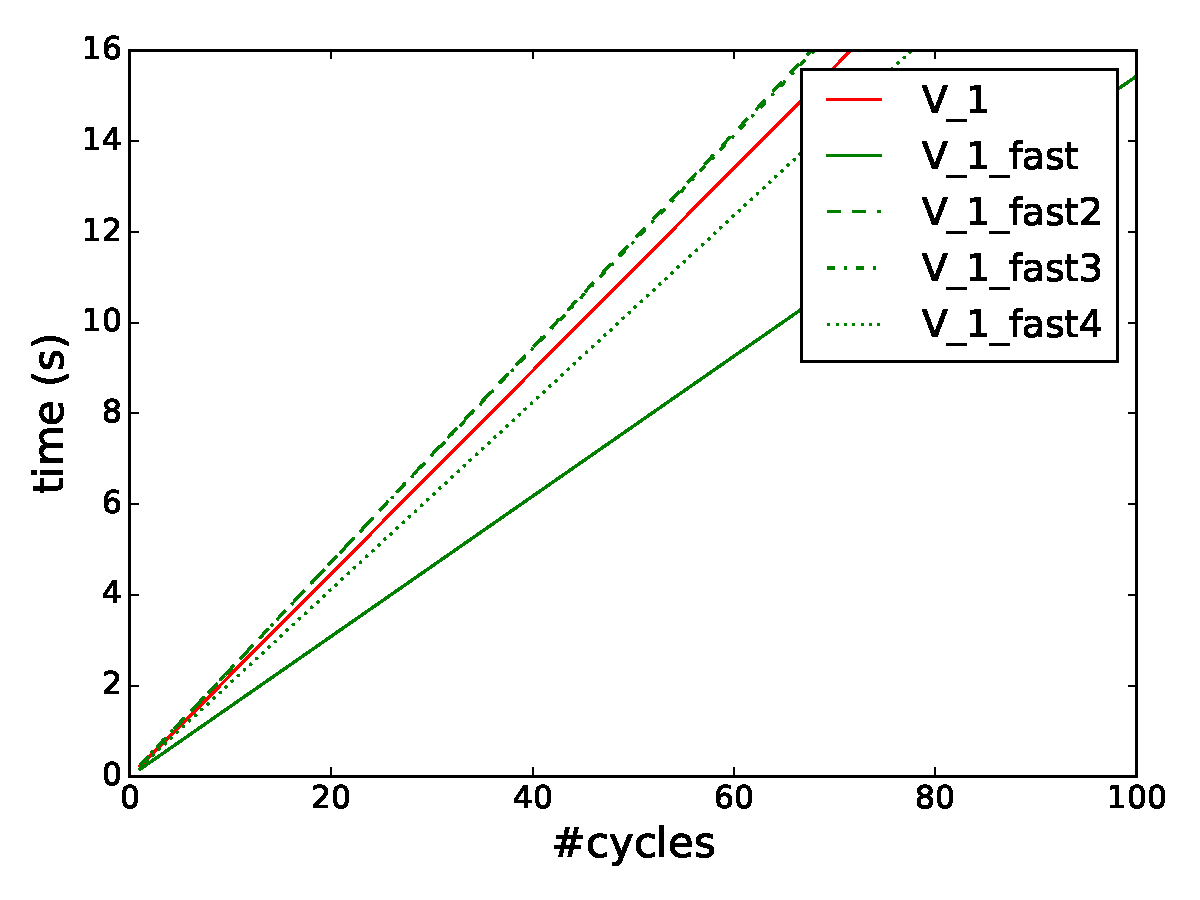
\includegraphics[width=0.33\linewidth]{figs/convergence_fast_time.pdf}
    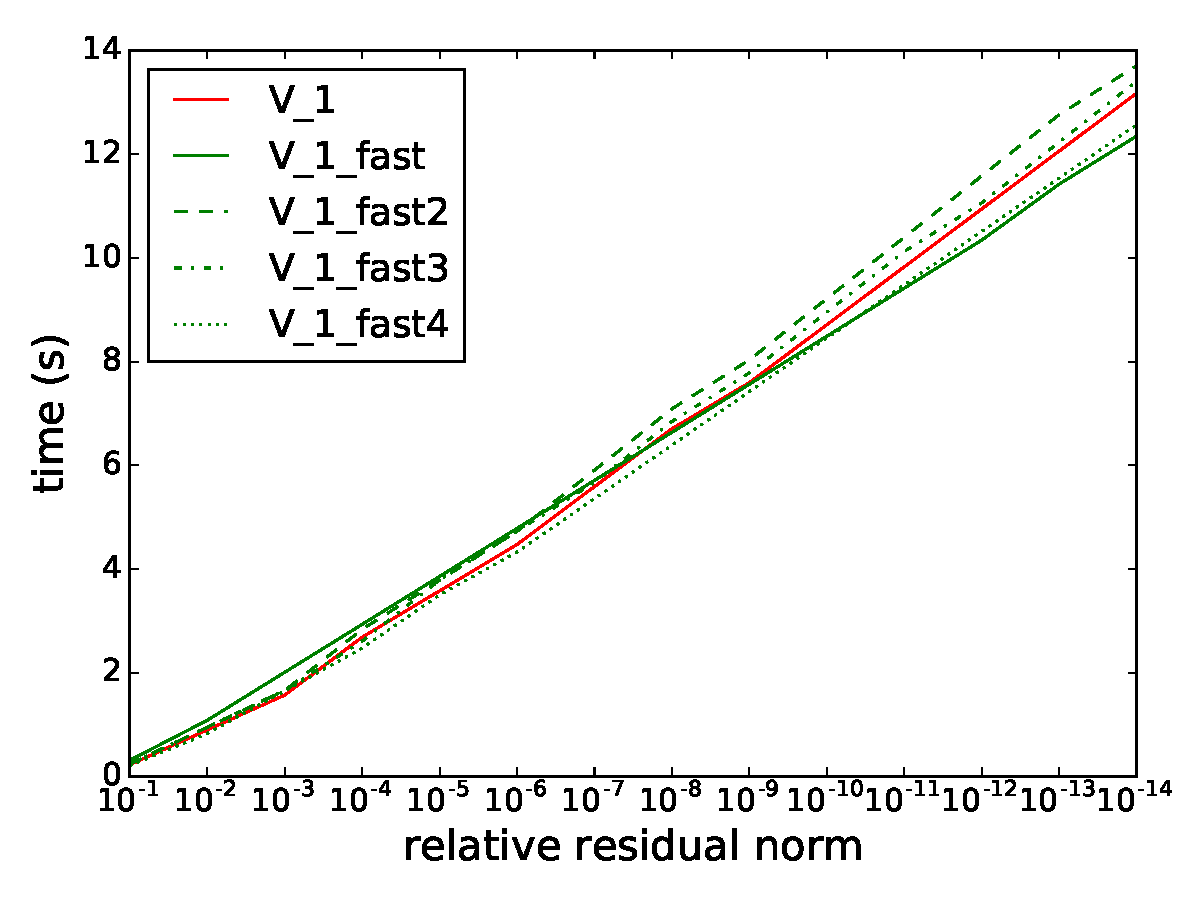
\includegraphics[width=0.33\linewidth]{figs/time_convergence_fast.pdf}
    \caption{Evaluation of 4 level-dependent relaxation tuning strategies.
    Residual norm per cycle (left), time spent in each cycle (middle) and
    convergence time in function of the error tolerance (right).}
    \label{fig.newstrat}
\end{figure*}

The strategy \emph{Fast} aims at reducing the cost of the cycle by removing the
penultimate relaxation which is very expensive, and expecting that the accuracy
lost at this point can be compensated by the relaxation at level 1.  The
strategy \emph{Fast2} executes a lot of relaxations at level 6, because it
should not increase by much the execution time of the V-cycle.  The reason to
choose level 6 instead of level 7 or 8 is that the relaxation at level 8 is
actually a direct solve. Thus, the result term is almost exact at level 7,
because the only source of error comes from the interpolation of $e^8$ (which
is exact) into $e^7$. This is why, we might expect better results by adding
relaxations at level 6. The strategy \emph{Fast3}, pushes the previous idea one
step further. If we assume that doing more than one relaxation gets a more
accurate error estimation at level $l$, then at level $l-1$ we do not need to
correct a lot by doing more relaxations. However at level $l-2$ we have been
through 2 interpolations since the last good estimation of the error vector,
therefore we increase the number of relaxations again. Since the first levels
are very expensive, we stop this recursion at level 3.  Finally, we propose one
last strategy \emph{Fast4} which is a softer version of \emph{Fast} where the
relaxation at level 3 is removed, producing a less accurate result at that
point, but expecting it can be compensated by the two relaxations at level 1
and 2.

%\begin{figure*}
%    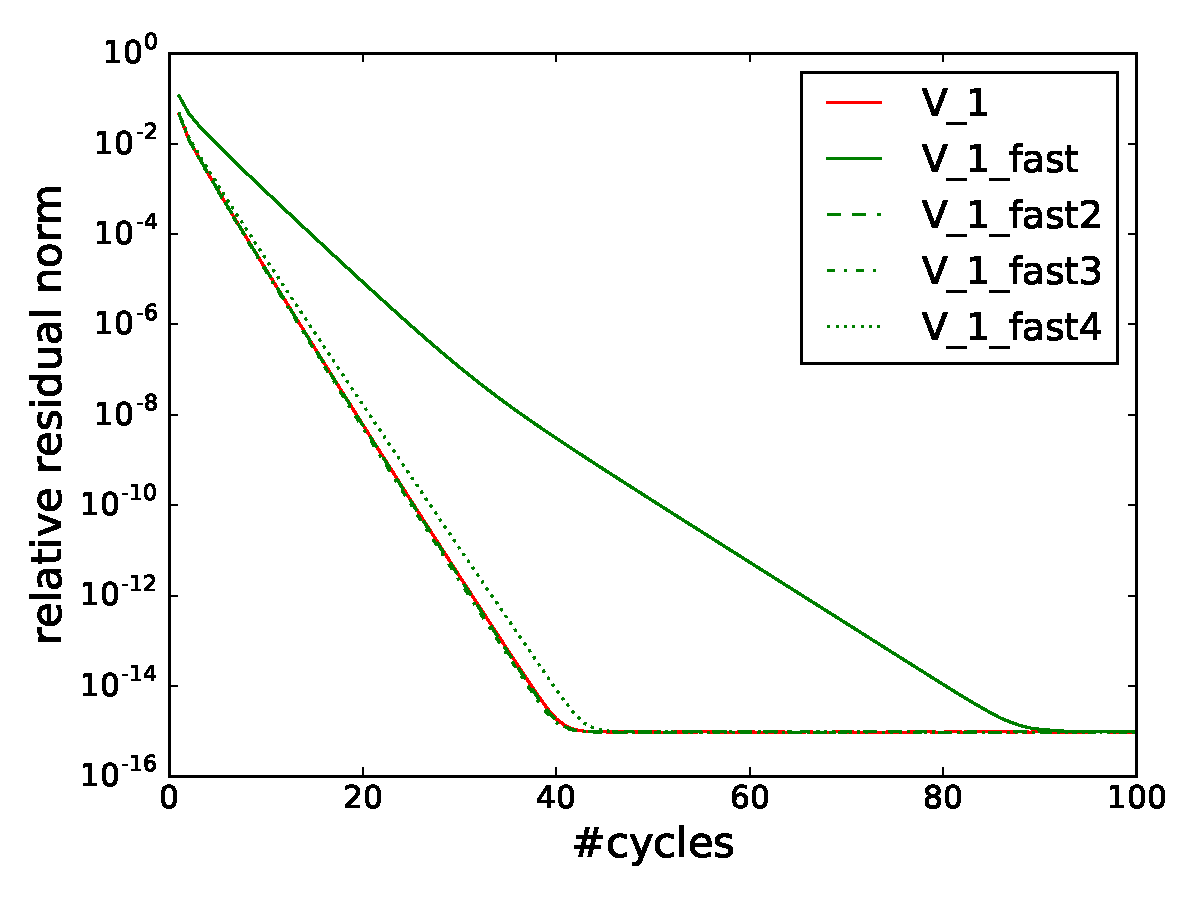
\includegraphics[width=0.33\linewidth]{figs/convergence_fast_small_norm.pdf}
%    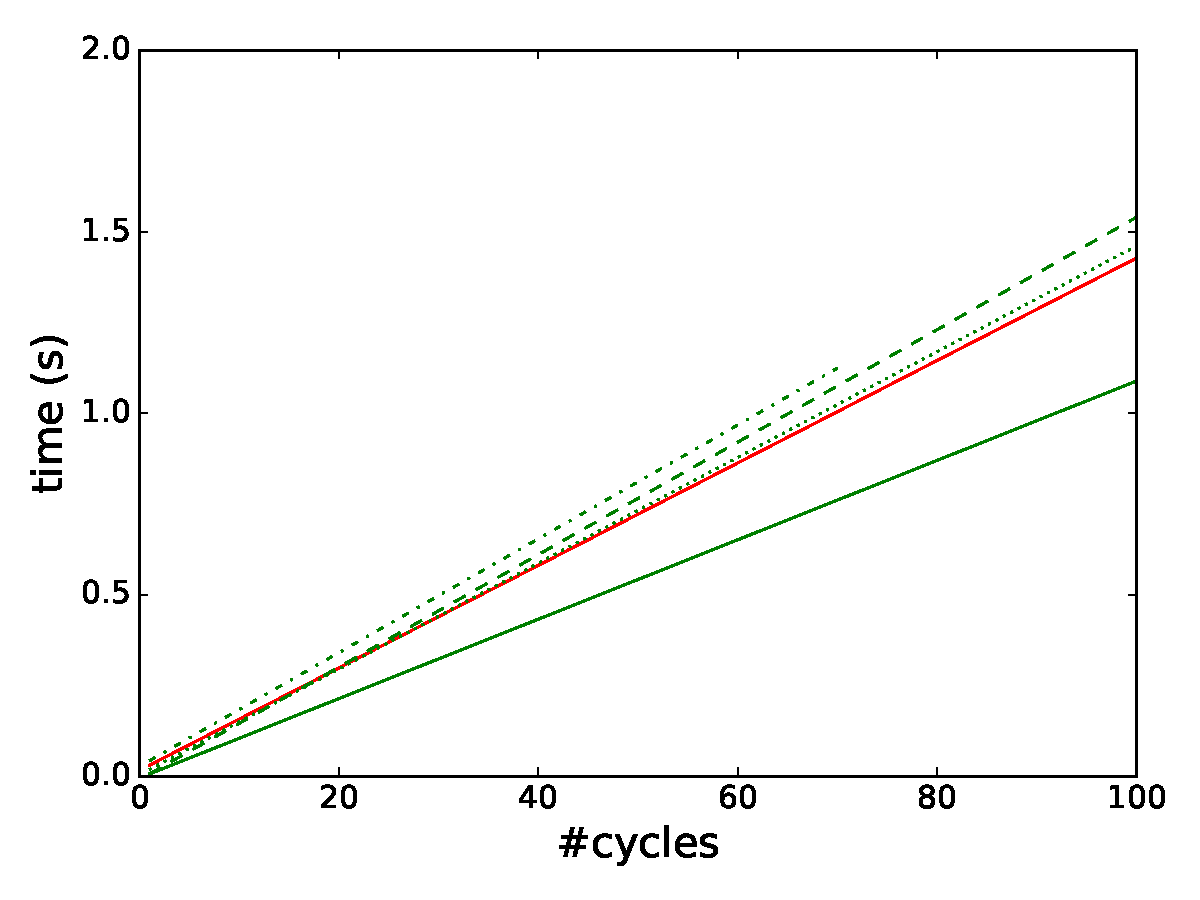
\includegraphics[width=0.33\linewidth]{figs/convergence_fast_small_time.pdf}
%    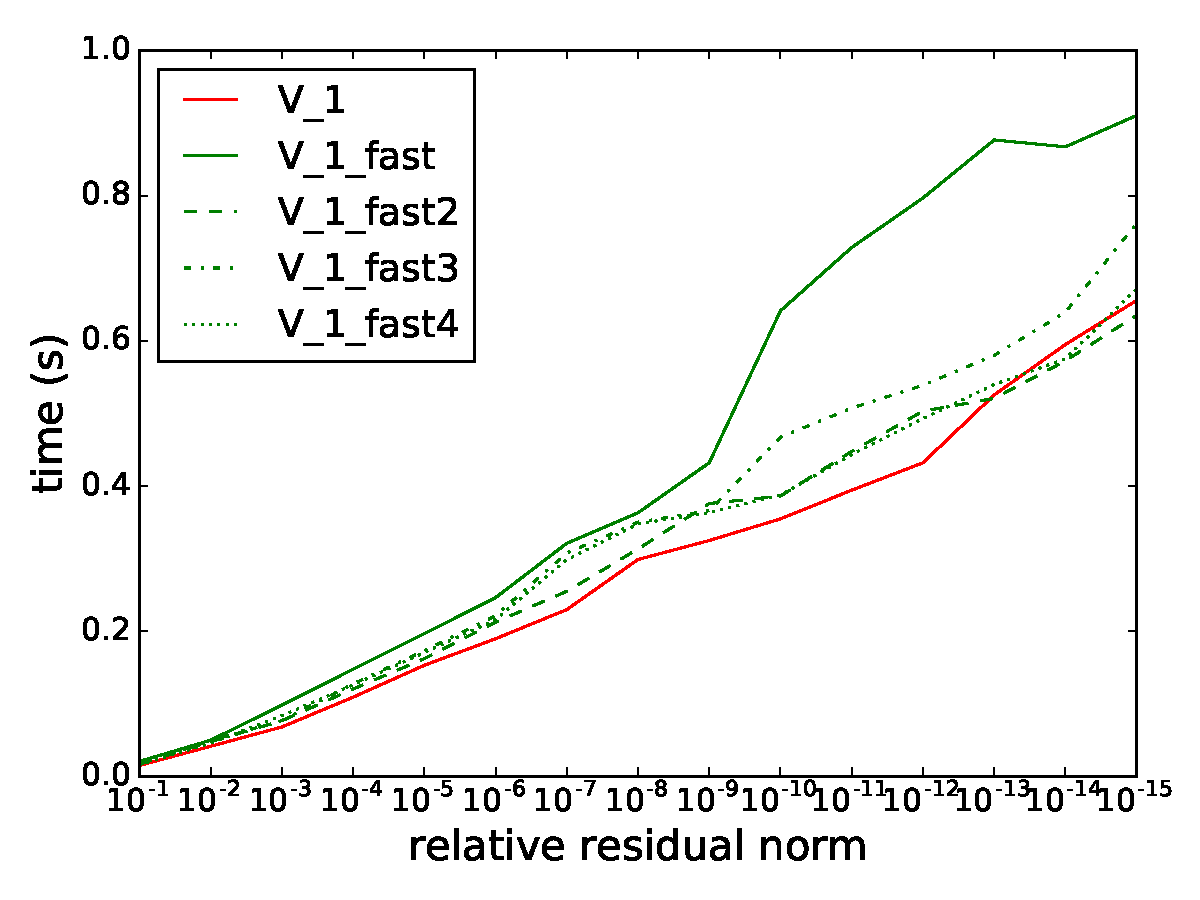
\includegraphics[width=0.33\linewidth]{figs/time_convergence_fast_small.pdf}
%    \caption{Final residual norm of the 4 new strategies per iteration (left),
%    interpolated execution time per iteration (middle) and convergence time as
%    a function of the tolerance (right) on a small matrix.}
%    \label{fig.newstrat_small}
%\end{figure*}

We evaluated these 4 proposed strategies in the original $512,000\times
512,000$ matrix.  The results are shown in Figure~\ref{fig.newstrat}.  The
first thing to observe is that removing the relaxation at level 2 (i.e. the \emph{Fast} approach) does not
provide any benefit. It does save time during each cycle but the accuracy loss
per cycle is too high (i.e., more
cycles needed for convergence), leading to a convergence rate close to the baseline configuration. 
The other thing to notice is that adding more
relaxations in the last levels slightly increases the execution time but it
does not provide any benefit on the accuracy side. Thus, strategies
\emph{Fast2} and \emph{Fast3} are not really efficient.  Overall, strategy \emph{Fast} and strategy
\emph{Fast4} seem to be more or less equivalent to the original V cycle as it
reduces a bit the cost of each cycle and the convergence rate per cycle is also
slightly smaller.  More tests were performed on a smaller matrix with an
initial matrix size of 64,000 with only a 6-level grid. The results were
similar (all strategies except \emph{Fast4} were less efficient than the original algorithm) and are not shown in this paper for brevity.


%We find again that the original V cycle seems to be the best as \emph{Fast3}
%converges in slightly less cycles, but this strategy is clearly too expensive
%with a bigger matrix so overall it is not as efficient as the baseline.


\subsection{An Asymmetric Strategy}
\label{sec.assymetric}

In the previous section, we observed no big improvement compared to the
original V-cycle with 1 relaxation at each level, except for strategy
\emph{Fast4} which did show some slight improvement. Initially, we applied the
same number of relaxations at all levels; then we tried different numbers of
relaxations for different levels. However, all these strategies share something
in common: for a given level they do the same number of relaxations when going
down or up in the cycle, following a very symmetric behaviour.

In contrast, the main idea behind a MG algorithm is rather asymmetric. More
precisely, in MG algorithms the types of computations performed when moving to
a coarser grid level are different than the type of computations done when
going back to a finer grid level. In the first case, the objective is to
compute a first approximate solution to the current system while in the second
case the objective is to refine the error term. In other terms, we first
compute an approximation at level $l$, then we use the level $l+1$ to compute
an approximate error term $e^l$ and finally we redo some relaxation to refine
the solution. The two relaxations do not have the same goal.

This analysis opens the door for strategies in which grid levels have a
different number of relaxations when going down than when going up in the
cycle.  In fact, assuming that the values of the error vectors are smaller
than a given $\epsilon$ from the exact value after just a relaxation step, one
would not need to do a relaxation before computing the approximate error term
for the next level, but just compute directly the error term when going back up
in the cycle. In other words, the relaxations done when going up could
potentially compensate inaccuracies obtained after removing relaxations when
going down. From that idea we define a new asymmetric strategy: we use a
V-cycle in which we do one relaxation at each level only when we are going up
in the cycle (i.e., no relaxations when going down).  We call this strategy
\emph{Up}.

We run \emph{Up} and \emph{Fast4}, as long as the classical V-cycle, on the
same matrix of size 512,000. For generality purposes, this time we also
evaluate matrices generated from other physical problems: i) 3D Laplace equation with a 9-pt stencil (with $c_x,c_y,c_z$ anisotropy parameters), ii) 3D Laplace
with a 27-point stencil, and another iii) 3D partial derivative equation with
Dirichlet boundary conditions. All problems use the same size of matrix. The
results are presented in Figure~\ref{fig.up_comparison}.

\begin{figure*}
    \centering
    \subfloat[\textsc{Unstructured-Anisotropy}]{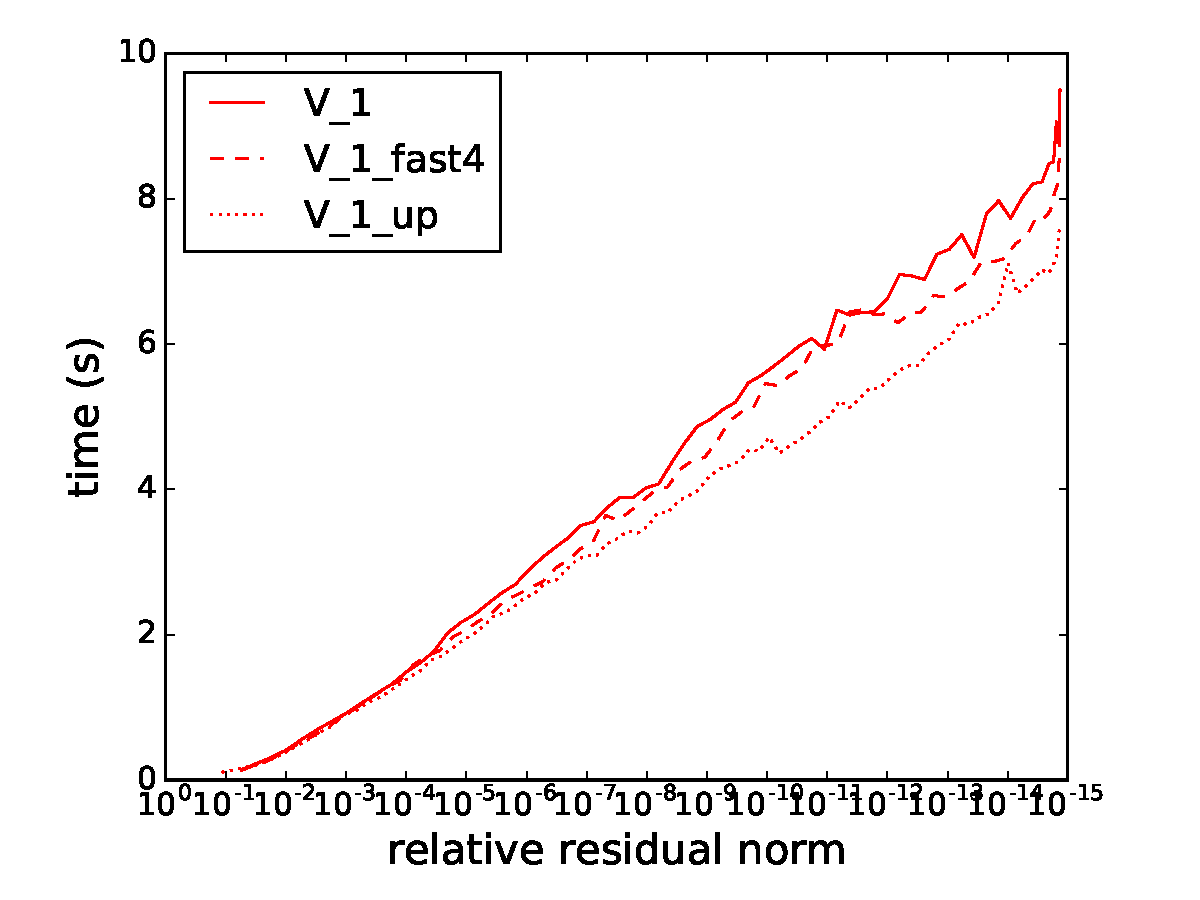
\includegraphics[width=0.45\linewidth]{figs/time_convergence_up_1.pdf}}
    \subfloat[\textsc{3DLaplace-9pt(1,1,1)}]{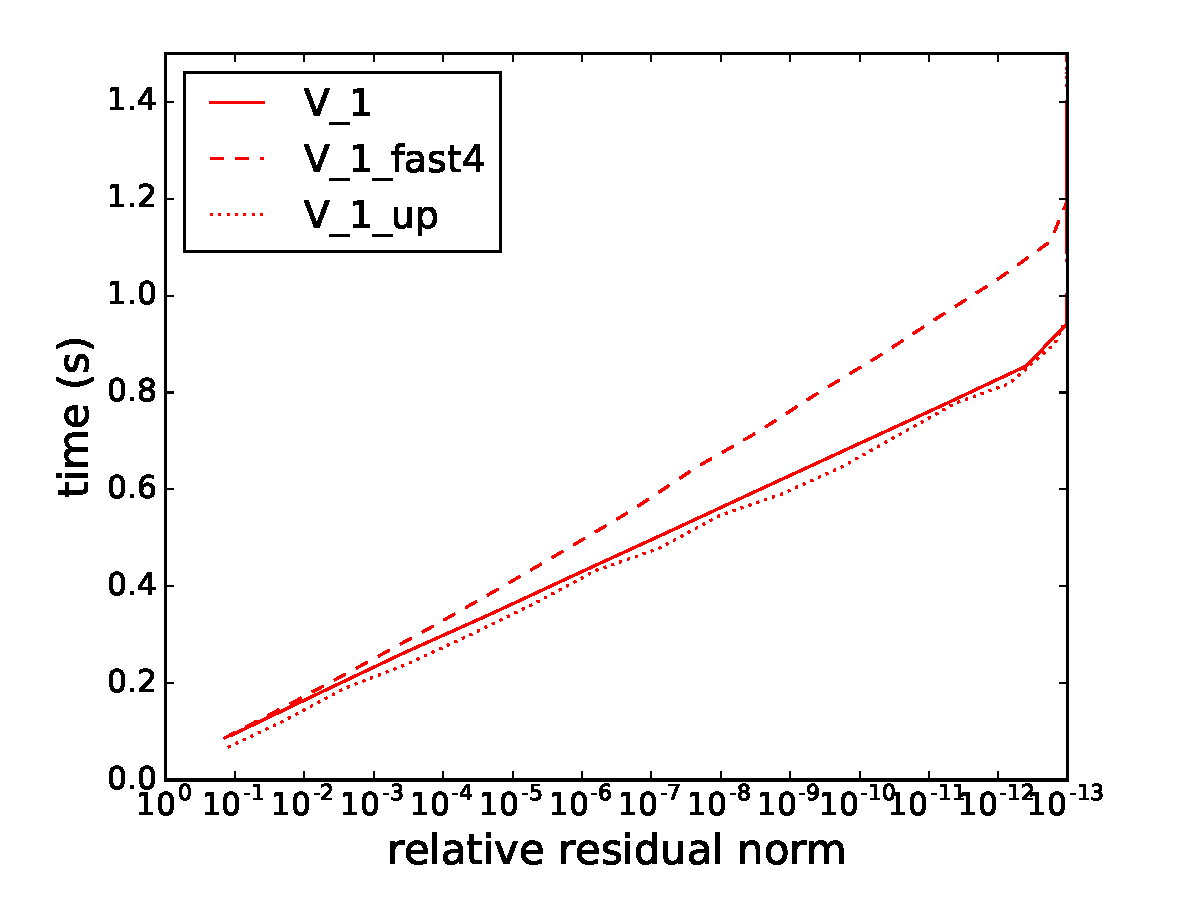
\includegraphics[width=0.45\linewidth]{figs/time_convergence_up_2.pdf}}\\
    \subfloat[\textsc{3DLaplace-9pt(0.1,0.1,0.01)}]{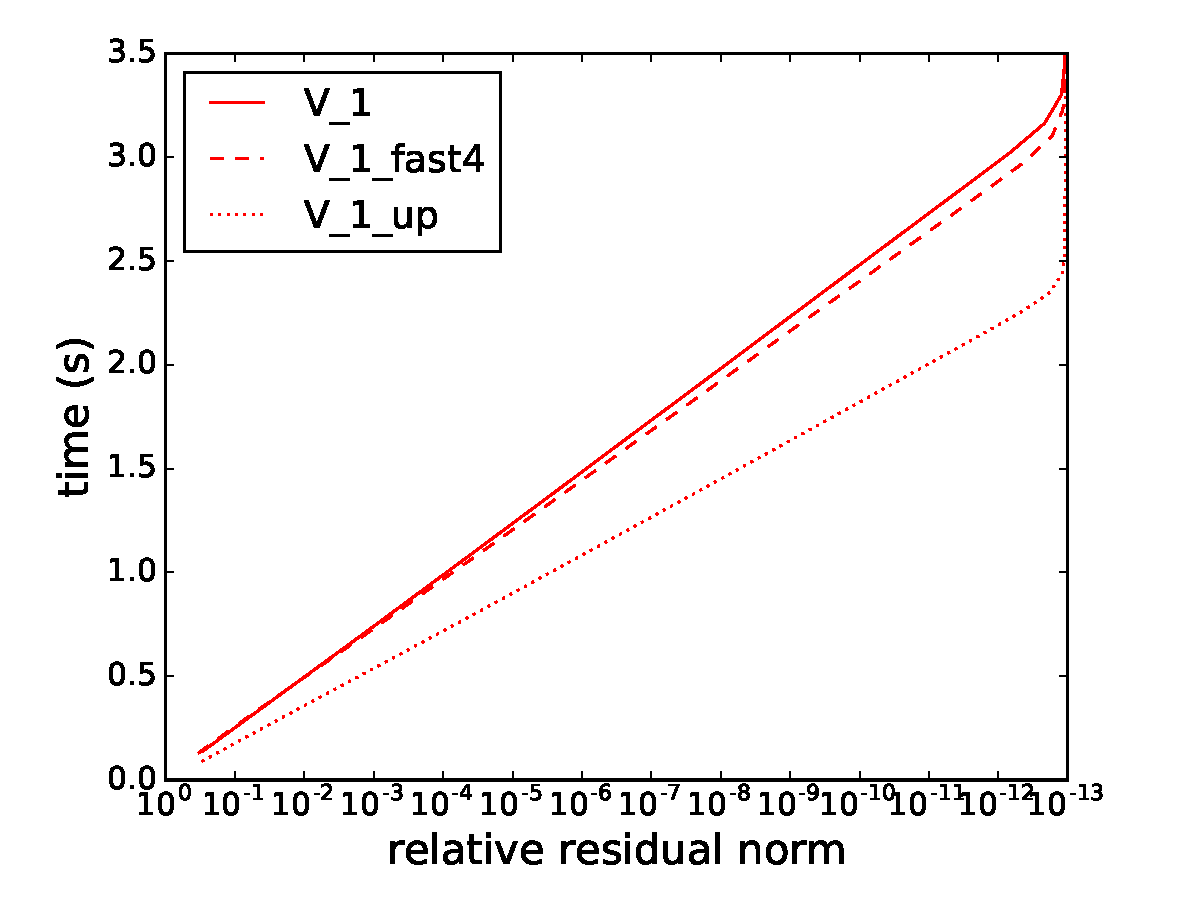
\includegraphics[width=0.45\linewidth]{figs/time_convergence_up_5.pdf}}
    \subfloat[\textsc{3DLaplace-9pt(5,5,5)}]{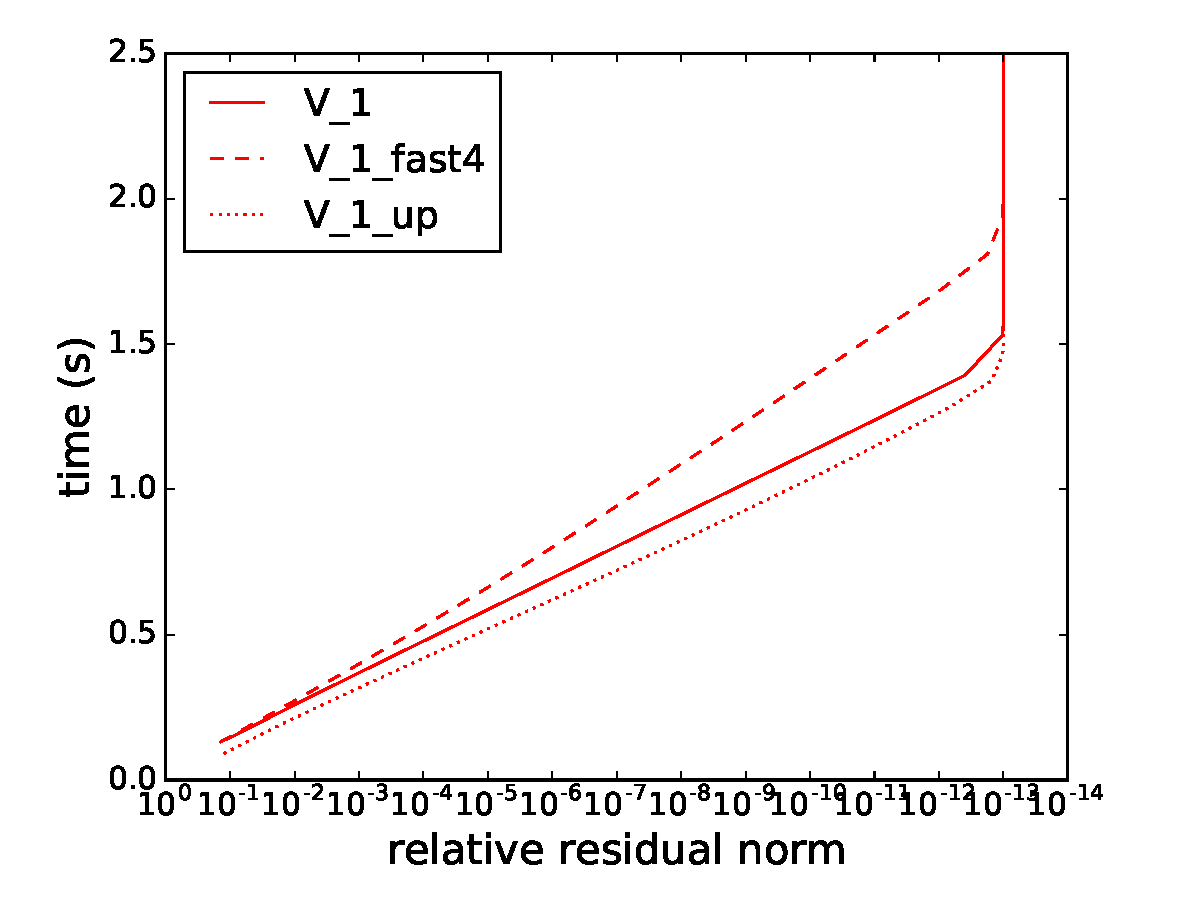
\includegraphics[width=0.45\linewidth]{figs/time_convergence_up_6.pdf}}\\
    \subfloat[\textsc{3DLaplace-27pt}]{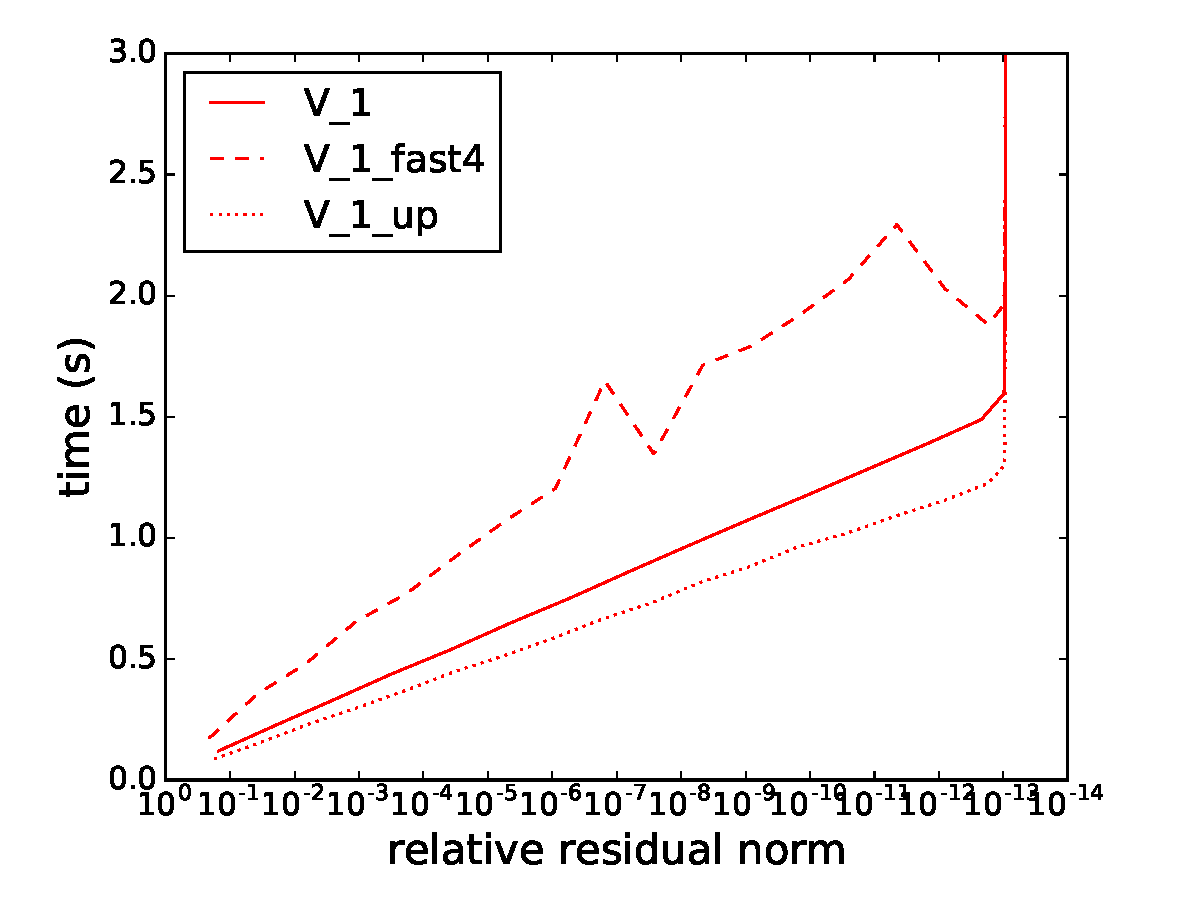
\includegraphics[width=0.45\linewidth]{figs/time_convergence_up_3.pdf}}
    \subfloat[\textsc{PDE-Dirichlet}]{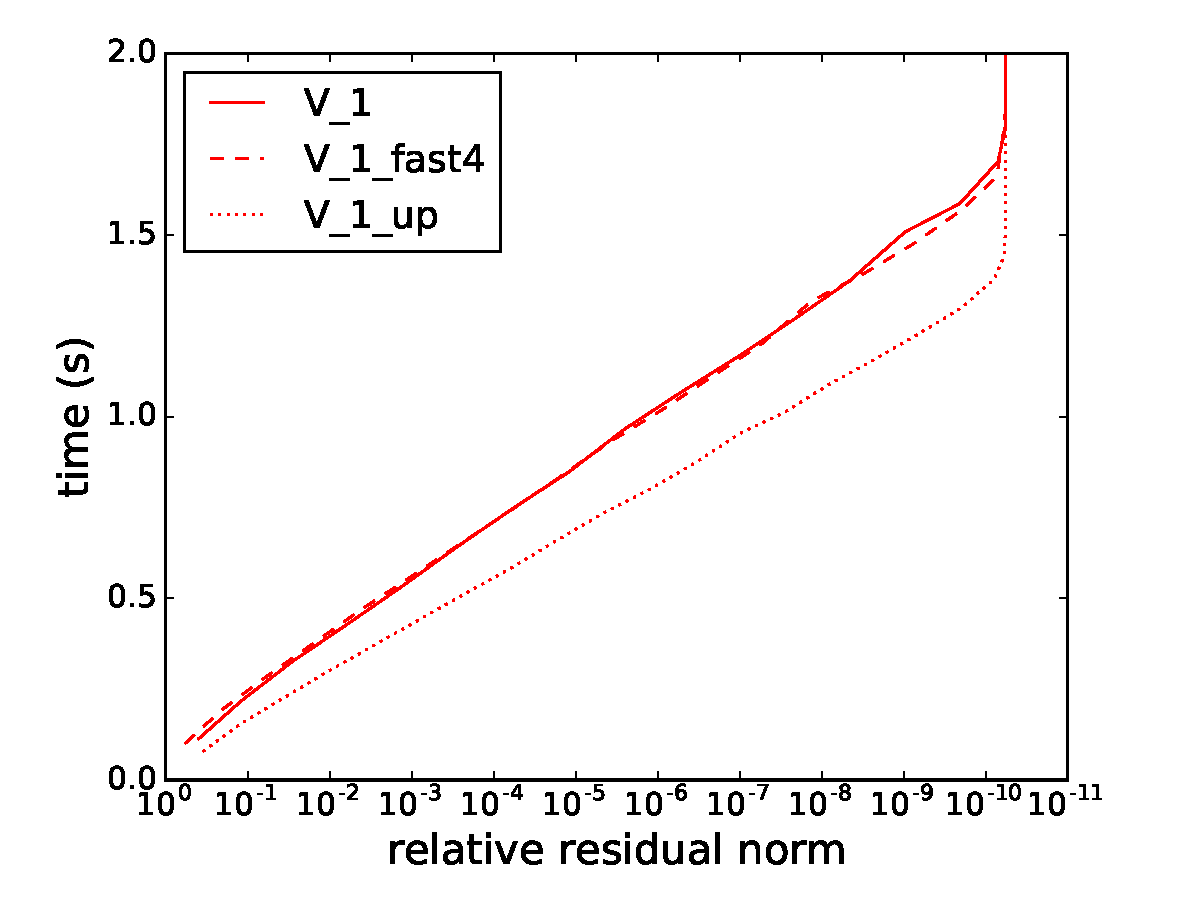
\includegraphics[width=0.45\linewidth]{figs/time_convergence_up_4.pdf}}
    \caption{Comparison of the original algorithm V1 with \emph{Fast4} and \emph{Up} strategies.}
    \label{fig.up_comparison}
\end{figure*}

The first thing we observe is that the \emph{Fast4} strategy does not
always perform well. In fact, for two of these four applications the
convergence rate is significantly slower than the classic V1 strategy.
However, the \emph{Up} strategy seems to be quite efficient; it improves
convergence speed by $12\%$,$7\%$,$20\%$ and $22\%$ for
\textsc{Unstructured-Anisotropy}, \textsc{3DLaplace-9pt},
\textsc{3DLaplace-27pt(1,1,1)} and \textsc{PDE-Dirichlet} respectively.

Given these positive results, we extended further our evaluation from
single-node runs to distributed executions in multiple nodes, in order to test
the viability of the \emph{Up} strategy when the algorithm is parallelized and
distributed. Larger cases were tested on a cluster with 100 compute nodes, 
each node equippred with 2 Intel Xeon E5-2630 v3 Haswell 8-core processors, 
each core at 2.4 GHz, and with 20 MB L3 cache.
%Each node is equipped with 2 Intel processors, 2 nvidia GPUs, over 20GB of DRAM
%and all connected through an Infiniband network.}

The total size of the matrix is set to either 5,832,000 or 13,824,000, while
the topology is composed of either 27 (3x3x3), 36 (6x6x1) or 64 (4x4x4)
processors, where each processor holds 1 MPI process and runs 1 OpenMP
thread per process. The problems tested are \textsc{3DLaplace-9pt} and
\textsc{3DLaplace-27pt}.  For these 6 possible combinations, we observe an
average improvement of 18.4\% (ranging from 16.0\% to 28.3\%) for
\textsc{3DLaplace-9pt} and 20.5\% (ranging from 16.2\% to 25.0\%) for
\textsc{3DLaplace-27pt}. It seems that \emph{Up} outperforms the
classical V-cycle even more when the problem size increases, but seems to cap at around
25\% improvement. Figure~\ref{fig.mtup} presents the results for the matrix
size 13,824,000 and \textsc{3DLaplace-27pt}, for the 3 different processor
topologies. Similar results are obtained for the other applications but are not
shown here for brevity.

\begin{figure*}[t]
    \subfloat[3x3x3]{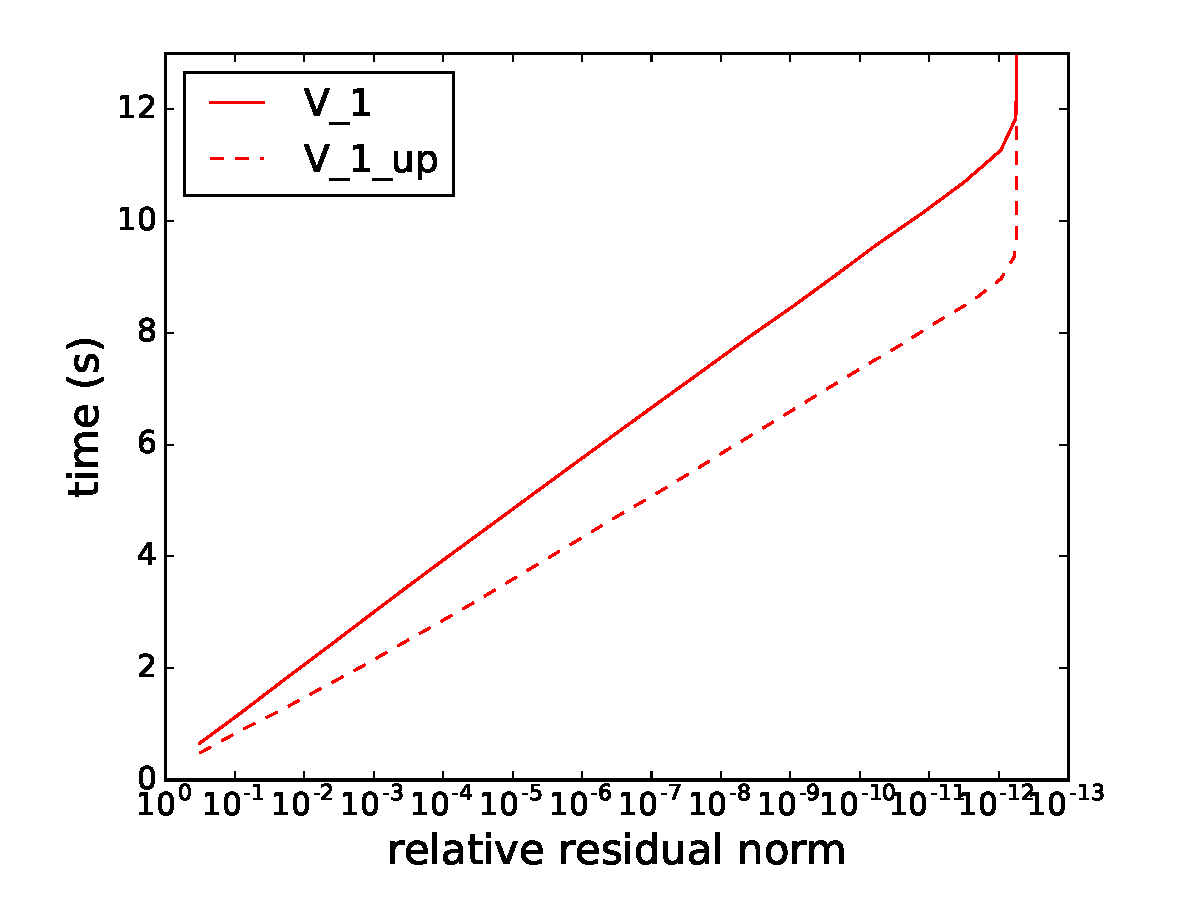
\includegraphics[width=0.33\linewidth]{figs/mt_27.pdf}}
    \subfloat[6x6x1]{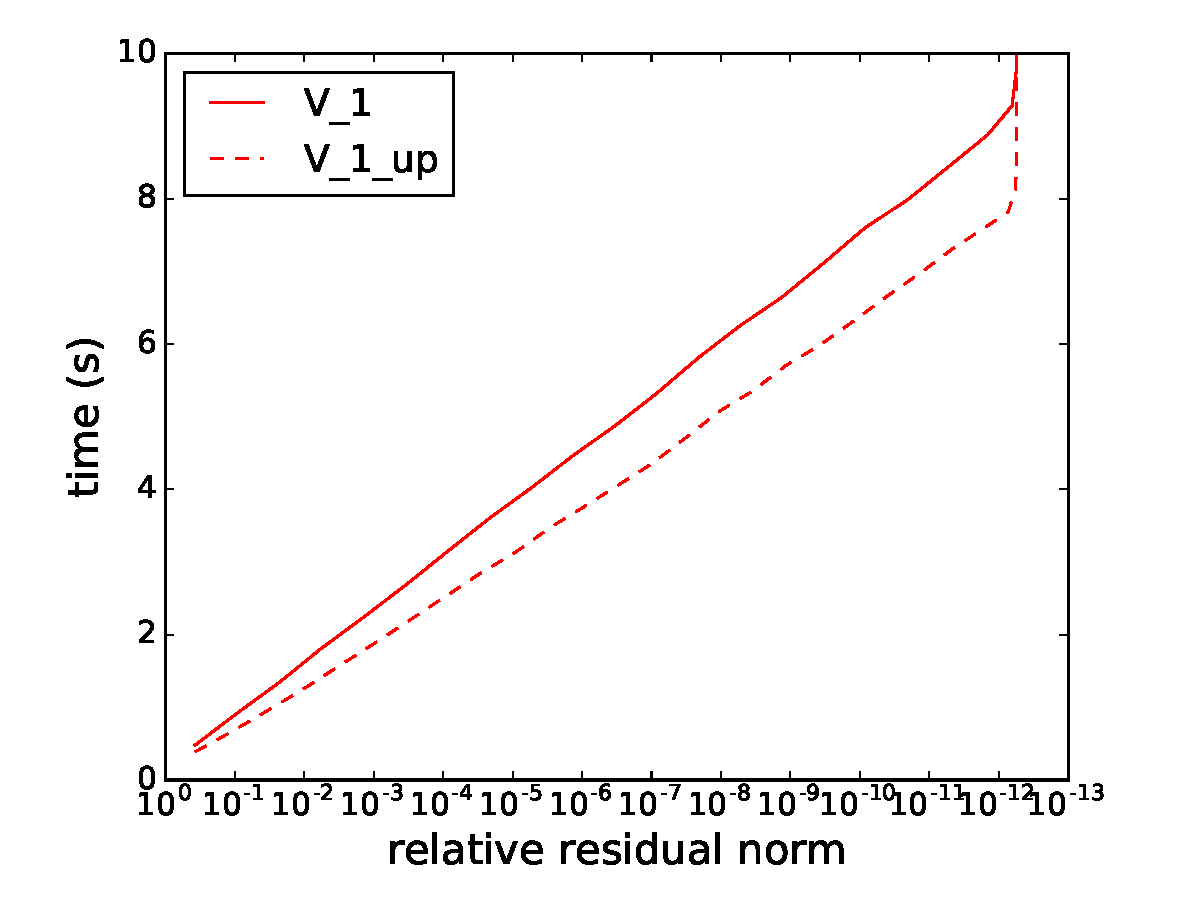
\includegraphics[width=0.33\linewidth]{figs/mt_36.pdf}}
    \subfloat[4x4x4]{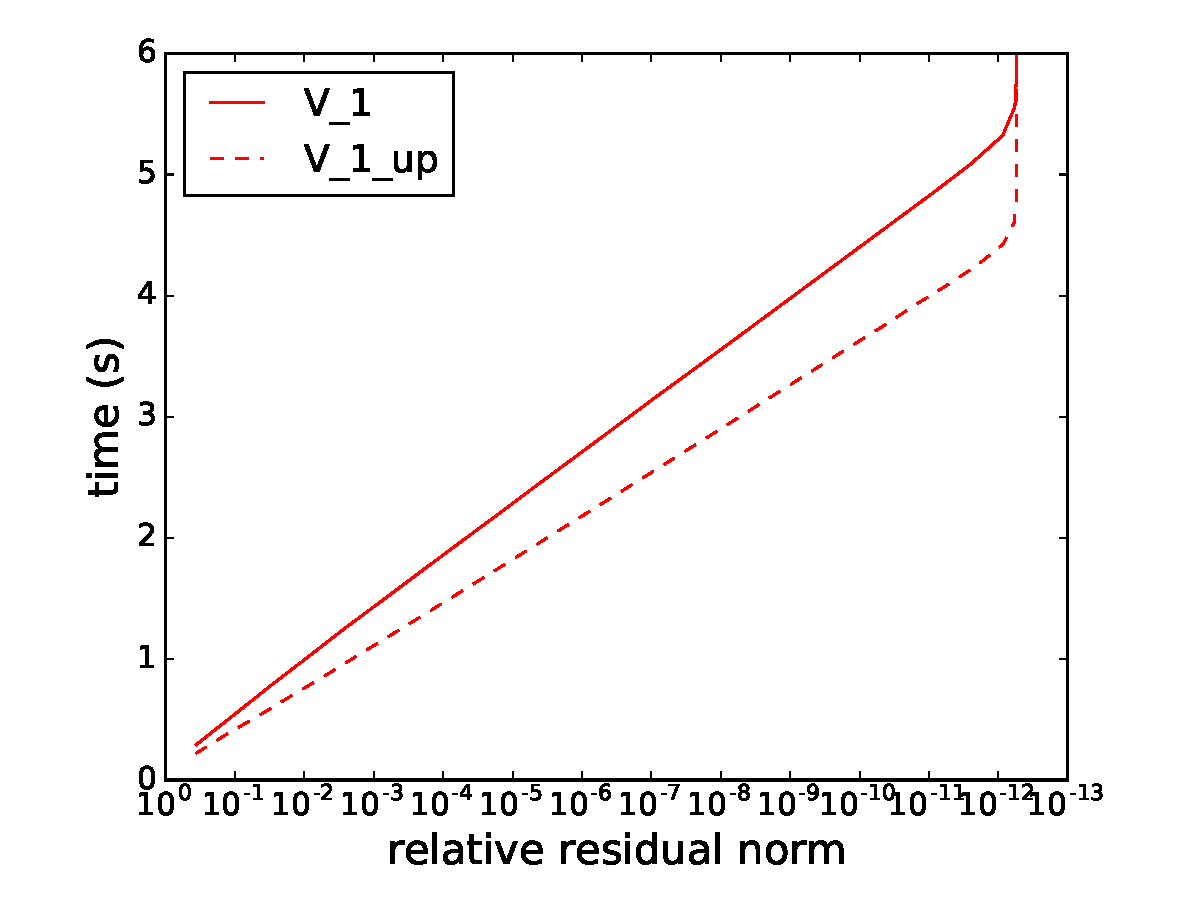
\includegraphics[width=0.33\linewidth]{figs/mt_64.pdf}}
    \caption{Comparison of original algorithm V1 with \emph{Up} strategy for
    \textsc{3DLaplace-27pt} on a 240x240x240 grid with different processor topologies.}
    \label{fig.mtup}
\end{figure*}




%% Section IV
\section{Precision-Performance Optimizations}
\label{sec:precision}

\subsection{A new version of multi-grid algorithm}

Observing the initial results presented on Figure~\ref{fig.first_tests},
one can notice that independently of how many relaxations are performed, or
which cycle shape is used, and more importantly, of how many cycles are
executed, the residual norm of the algorithm reaches a lower bound (it is
around $10^{-15}$). This bound comes from the internal limitations of the
\texttt{double} floating-point representation.  Indeed, a double uses 8 bytes
(52 bits for the mantissa, 11 for the exponent and 1 bit for the sign).
Naturally, a space-constrained representation does not allow a full description
of all rational numbers (for example between $2^{52}$ and $2^{53}$ only
integers can be represented).  If we increase the number of bits used in the
representation we can describe more and more numbers. Similarly, if we reduce
the number of bits used in the representation, we lose accuracy for numbers
that are not fully representable.

The advantage of using lower precision for the floating point operations is a
faster and more energy-efficient computation. \leo{The reason for these gains
is that floating-point units (FPUs) require more circuit logic (silicon for
ASICs, LABs/DSPs for FPGAs) for high precision operators (the required area for a FPU increases at least linearly with the number of bits~\cite{govindu:2003}). FPUs Thus, reducing
precision allows more low precision FPUs, which increases the Instruction-Level
Parallelism (ILP) or Vectorization that the processor can reach, hence
increasing its peak performance.}

\leo{Considering our algorithm, lower precision computations could be used if
the required accuracy allows it. For instance, if the final result should have
an accuracy} of only $10^{-3}$ then the 64 bits \texttt{double} floating-point
representation is not needed to reach it, a lower precision is enough.
Moreover, analysing the presented results, it seems clear than during the first
cycles the accuracy is low and it does not require the full precision offered by
the double floating-point representation. This observation opens the door for
making use of lower precisions temporarily during the first cycles. Therefore, it
is important to study the impact of precision on performance for MG algorithms.

\leo{To study the trade-off between precision and performance,} we modify the
relaxations step of the algorithm (note that it is the more time consuming
part of the algorithm). In this function we can find 13 internal variables that
are originally of type \texttt{double}: 5 arrays and 8 scalars. We then propose
the following two modified versions of the MG algorithm.

\begin{itemize}

    \item \textbf{AMGfloat}, which changes the type of the 13 variables from
        \texttt{double*} or \texttt{double} to \texttt{float*} or
        \texttt{float}.

    \item \textbf{AMGmpfr(b)}, which makes use of the library
        MPFR~\cite{MPFR,MPFR_link} that introduces a type \texttt{mpfr\_t}.
        This type has a parameter $b$ which is the number of bits used in the
        mantissa of the variable. Every computation is done first in full
        precision and then rounded to a number with a mantissa using the number
        of bits given as parameter. In this version of the algorithm \emph{AMG}
        the 8 scalar variables of the relaxation function are replaced by
        \texttt{mpfr\_t} variables, all using the same number of $b$ bits for
        the mantissa.

\end{itemize}

Finally, we will denote by \emph{AMG} this original algorithm.  In terms of
arithmetic precision, \emph{AMG} behaves similarly to \emph{AMGmpfr(53)} and
\emph{AMGfloat} to \emph{AMGmpfr(24)}. There can be small differences depending
on the rounding method used.

Figure~\ref{fig.bits_accuracy} shows the accuracy that can be reached with
\emph{AMGmpfr(8)}, \emph{AMGmpfr(16)}, \emph{AMGfloat}, \emph{AMGmpfr(32)} or
\emph{AMGmpfr(64)}. The problem used is \textsc{Unstructured-Anisotropy}, with
2x2x2 processor topology and 20x20x20 matrix size. What we actually see on this
figure is the lower bound reached depending on the number of bits used.
However, before reaching this lower bound, all precisions show the same
accuracy. This means that, for example, while the accuracy of the solution is
below the threshold using single precision (32 bits), using 32 or a greater
precision to do the same computations will result in the same accuracy.
However, we expect single precision computations to be more efficient than
higher precisions in terms of time, space and energy.

\begin{figure}[htb]
    \centering
    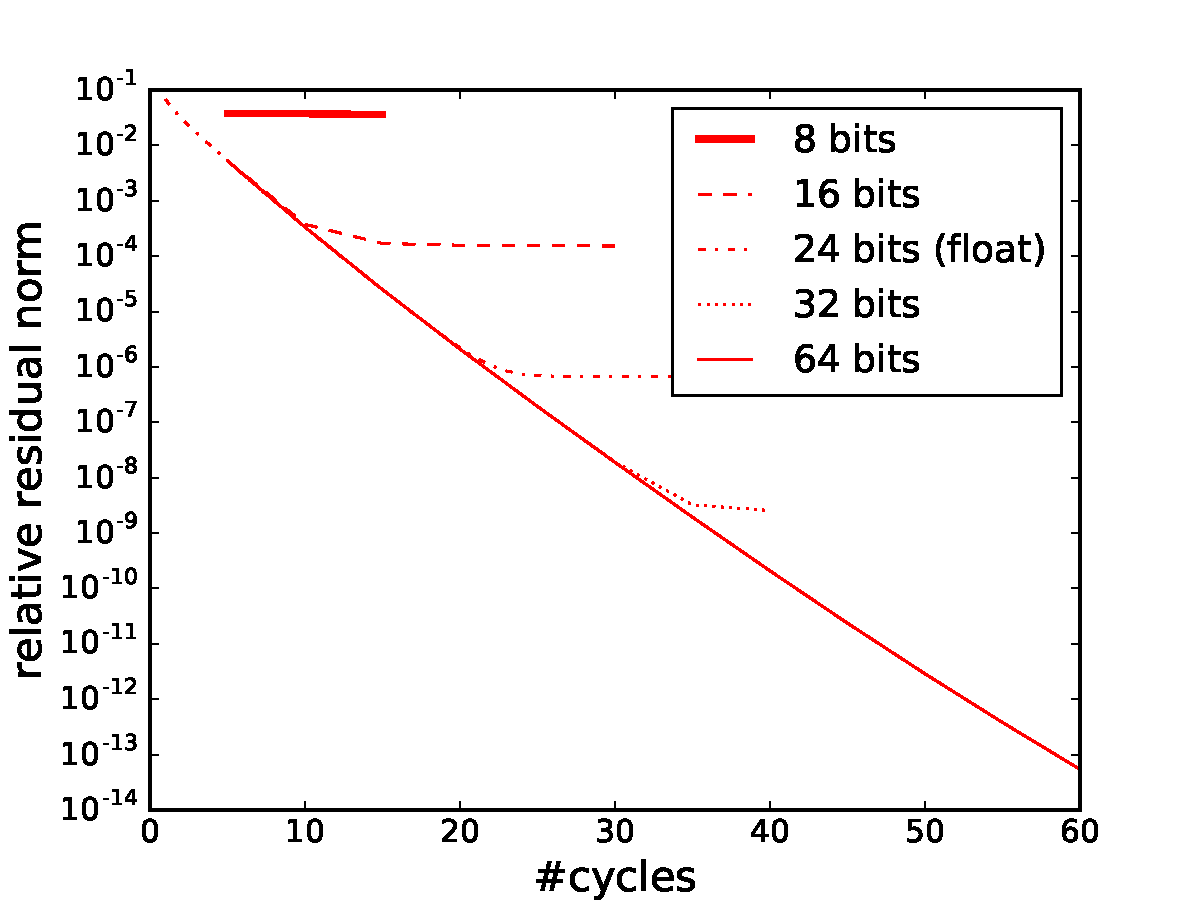
\includegraphics[width=0.9\linewidth]{figs/bits_convergence.pdf}
    \caption{Accuracy for different number of mantissa bits.}
%    Points (except for 24 bits) were obtained only for multiples of 5
%    iterations, but it is enough to see the thresholds appear.}
    \label{fig.bits_accuracy}
\end{figure}

The second thing we observe is that \emph{AMGfloat} 
behaves exactly as what we would expect from
\emph{AMGmpfr(24)} in terms of accuracy: it shows the same accuracy as versions
with more precision in the beginning, then it reaches a threshold between that
of \emph{AMGmpfr(16)} and that of \emph{AMGmpfr(32)}. It is important to
notice that in the \emph{AMGfloat} version more variables were changed from
\texttt{double} to \texttt{float}, however in the \emph{AMGmpfr(24)} version we
do not observe more accuracy degradation. This is because only a few
variables from the 8 scalars control the final precision as they are temporary
variables used for intermediate computations before being plugged back into the
input matrix/vector.

Given this analysis, we design a new algorithm that adapts the precision of the
variables during the execution. It is close to the \emph{AMGmpfr(b)} technique
except this time the precision can change between two cycles.  We fix a
threshold on the ratio between the relative residual norm of two consecutive
steps to trigger the precision change if the gradient is lower than the
threshold (i.e., limited gain in accuracy between two consecutive cycles). Then,
we define the following 3 strategies.

\begin{itemize}

    \item start at $b=16$ and do $b=b+8$ on threshold

    \item start at $b=32$ and do $b=b+8$ on threshold

    \item start at $b=16$ and do $b=b\times2$ on threshold

\end{itemize}

We run these strategies on a 240x240x240 matrix size with a 3x3x3 topology for
\textsc{3DLaplace-27pt}. Figure~\ref{fig.prec_incr} presents the evolution of
accuracy for the original algorithm and the 3 new adaptive strategies
introduced.  We see some steps appear, corresponding to the lower bound on the
accuracy at the current precision. Then, the precision is adapted to be able to
improve the overall accuracy. Even if we lose some accuracy when waiting for
the ratio between two consecutive relative residual norms to reach the
threshold; when the precision changes the convergence rate is more important
(for one cycle) than that of the original double-precision algorithm (i.e. the
slope is bigger), allowing the adaptive strategies to quickly \emph{catch-up}
any accuracy loss and reach the maximum accuracy (of $4.7\times 10^{-13}$) in
the same number of cycles as the original full precision algorithm (20-21
cycles).

\begin{figure}[htb]
    \centering
    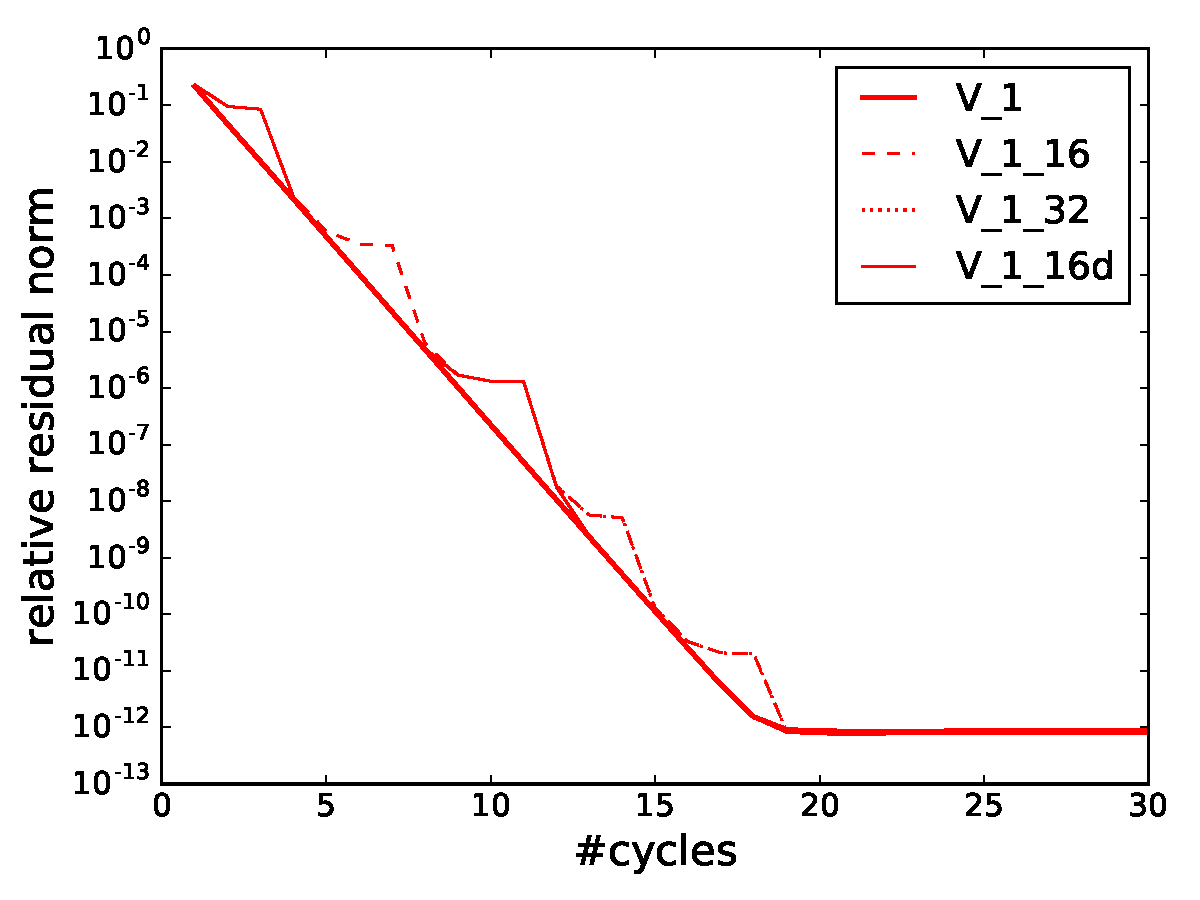
\includegraphics[width=0.9\linewidth]{figs/prec_incr.pdf}
    \caption{Accuracy of adaptive algorithms compared to the original
    double-precision with a precision threshold of $0.8$.}
    \label{fig.prec_incr}
\end{figure}

These results demonstrate that adaptive precision can be used to reach the
same accuracy in the same number of cycles, while each cycle is expected to be
less energy and time consuming because of lower precision. At this point two
questions arise. How to evaluate the energy/time savings of this adaptive
algorithm in a hypothetical hardware with multiple precisions available? Which
precisions should be used to maximize these savings? The complexity to answer
these questions comes from the fact that the MPFR library used to do these
accuracy experiments introduces a huge overhead in the computation. For
instance, running \emph{AMGmpfr(53)} is about 20 times more time consuming than
running the classic \emph{AMG}, whereas it represents the same double-precision
algorithm.  Moreover, this overhead is not influenced by the choice of the
number of bits. Therefore, we cannot use the execution times of the
computations done with MPFR as representatives of performance differences at
different precisions.




   \subsection{Optimal set of precisions}
   
   In this subsection, we provide an optimal set of precisions to minimize the total execution time, under the assumption that the time evolves linearly with $b$ the number of precision bits: $T(b) = \alpha b + c$.
   
   \begin{theorem}
     Given $b_{max}$, a maximum number of bits, $n$ the number of different precisions $b_1,\dots,b_n$ to use, and $T(b)=\alpha b+c$, with $\alpha$ and $c$ two constants, the time to execute a cycle at precision $b$, then
     the execution time of our adaptive algorithm is minimized for $b_i = \frac{i}{n}b_{max}$.
   \end{theorem}

   \begin{proof}
   From the previous experiments we can see that (i) the number of cycles needed to reach the lower bound for a given precision does not depend on the previous cycles (Figure~\ref{fig.prec_incr}), i.e.
if you start with cycles at precision $16$ then $32$, you will need the same number of cycles to reach the lower bound with $32$ bits as if you used only cycles with $32$ bits since the beginning of the algorithm; and that (ii) the number of cycles 
   needed to reach the lower bound is proportional to the number of bits $b$ used (Figure~\ref{fig.bits_accuracy}). We then define $\textsc{MaxIter}(b)$ the number of cycles needed so that the ratio between two consecutive
   relative residual norms is higher than a threshold $t$. We use the two observations to model $\textsc{MaxIter}(b) = \lfloor kb \rfloor$ for some constant $k$.
   Then we can compute the total execution time of the algorithm
   \begin{align*}
   T_{total}& = \textsc{MaxIter}(b_1)T(b_1)\\
   & +  \sum\limits_{i=1}^{n-1} (\textsc{MaxIter}(b_{i+1})-\textsc{MaxIter}(b_i))T(b_{i+1}).
   \end{align*}
   Indeed, when we reach the number of iterations $\textsc{MaxIter}(b_i)$ we change from precision $b_i$ to precision $b_{i+1}$.
   We can rewrite $T_{total}$ as
   \begin{align*}
    T_{total} &\approx k b_{1} T(b_1) + \sum\limits_{i=1}^{n-1} k(b_{i+1}-b_{i})T(b_{i+1})\\
	    & \approx k ( b_{n}T(n) + \sum\limits_{i=1}^{n-1} b_i ( T(b_i) - T(b_{i+1})).
   \end{align*}
   By plugging the expression of $T(b)$ into the previous equation and considering the maximum precision we want is $b_{max}=b_n$, we finally get:
   \begin{equation}
    T_{total}  = k\alpha\left(b_n^2 + \sum\limits_{i=1}^{n-1} (b_i^2 - b_i b_{i+1})\right) + kb_{max}c.
   \end{equation}
   
   Let us consider the function $f(x_1,\dots,x_n) = \sum\limits_{i=1}^n x_i^2 - \sum\limits_{i=1}^{n-1} x_ix_{i+1}$. Finding the minimum of $f(x_1,\dots,x_{n-1},1)$ will give
   us the minimum of the execution time.
   By simple partial derivation:
   \[ \frac{\partial f(x_1,\dots,x_n)}{\partial x_i} = 2x_i - (1-\delta_{i,n})x_{i+1} - (1-\delta_{i,1})x_{i-1} \]
   where $\delta_{a,b} $ is equal to 1 if and only if $a=b$, 0 otherwise.
   
   This is where the boundary condition $x_n = 1$ is useful: if we do not set it to a number different from 0, the function is minimized for $x_1=\dots=x_n=0$. This applied to our problem
   makes no sense, as we would't be doing any computation. The boundary condition represents the fact that we need to reach an existing precision ($b_{max}$) eventually. By a simple scaling,
   considering $1$ instead of $b_{max}$ makes computation easier and does not change the resolution of the the following system (up to a factor):
   
   \resizebox{0.9\linewidth}{!}{
   $\left\{
   \begin{tabular}{rcl cccccccccc cl}
    $\frac{\partial f(x_1,\dots,x_n)}{\partial x_1}$ & = & $2x_1$ & $-$ & $x_2$  &     &       & & 	 &&     &     &       & = & 0 \\
    $\frac{\partial f(x_1,\dots,x_n)}{\partial x_2}$ & = & $-x_1$ & $+$ & $2x_2$ & $-$ & $x_3$ & & 	 &&     &     &       & = & 0 \\
    & \vdots &&&&&&&&&&&&&\\
    $\frac{\partial f(x_1,\dots,x_{n})}{\partial x_{n-1}}$ & = &        &     &        &     &       & & $-x_{n-2}$ & $+$ & $2x_{n-1}$ & $-$ & $x_n$ & = & 0 \\
    $x_n$ & = & 1 &&&&&&&&&&&&\\
   \end{tabular} \right.$
  }
  
  Solving this system of equations is equivalent to solving the linear system $Ax=b$ where
  \[ A = \begin{bmatrix}
    2       & -1 &  &  &  \\
    -1       & 2 & -1 &  &  \\
    & \ddots & \ddots & \ddots & \\
    & & -1 & 2 & -1 \\
           &  &  & -1 & 2
\end{bmatrix} \textup{ and } b = \begin{bmatrix} 0 \\ \vdots \\ 0 \\ 1 \end{bmatrix} \]
   
   This system has a unique solution which is $\begin{bmatrix} \frac{1}{n} & \dots & \frac{n-1}{n} \end{bmatrix}$.
   The minimum of $f(x_1,\dots,x_n)$ with boundary condition $x_n=1$ is thus reached for $x_i = \frac{i}{n}$.
   It is, when multiplied by $b_{max}$, the solution that minimizes our total execution time.
   \end{proof}
   
   This proof holds only if the time evolves linearly with $b$, but \textit{we could also apply it to minimize the energy consumption} assuming that the energy consumption of one cycle increases linearly with $b$. The next section will investigate whether
   this assumption holds.

\subsection{Evaluation}

In order to estimate the cost of our algorithm, we want to model the time of an
iteration at precision $b$. We model an iteration by the following formula:
$an^3b^\alpha+c$, where $a,c$ and $\alpha$ are constants, $n$ is the size of
the problem and $b$ the number of bits. Indeed, we expect the time to be
proportional to the cube of the problem size as we deal with 3D problems, and
the parameter $\alpha$ will characterize how the time evolves when we double
the number of bits: if $\alpha = 1$, then multiplying by two the number of bits
will multiply by two the cost of an iteration (i.e., linear proportion). Maybe
the reality could be described by a more complicated polynomial in $b$, but we
want to keep the model simple enough and see if the data can fit it.


%    To provide numerical values for $a$,$\alpha$ and $\beta$, we measured the execution times of different scenarios. Each scenario computes 50 iterations on a 64x64x64 matrix, on different processor topologies, and using
%    either only single-precision floating point variables or only double-precision floating point variables. We denote by $x_{b,n}$ the empirical value obtained using $b$ bits and $n$ processors. Results are reported in Table~\ref{table.time_measure1}.
%    \iffalse
%    P1x1x1, 10 iterations, average on ten runs\\
%    \begin{tabular}{|l|c|c|c|c|}
%    \hline
%     \multirow{2}{*}{Experiment} & \multicolumn{2}{c|}{Single-Precision} & \multicolumn{2}{c|}{Double-precision} \\
%     \cline{2-5}
%     & Solve (s) & Cycle (ms) & Solve (s) & Cycle (ms) \\
%     \hline
%     (1) 40x40x40 & 1.308 & 12 & 1.543 & 14\\
%     \hline
%     (1) 80x80x80 & 10.794 & 100 & 13.033 & 121.5\\
%     \hline
%     (2) 20x20x20 & 0.1316 & 1.1 & 0.1411 & 1.2 \\
%     \hline
%     (2) 40x40x40 & 1.026 & 9.5 & 1.195 & 11 \\
%     \hline
%     (2) 80x80x80 & 8.068 & 74 & 9.595 & 88 \\
%     \hline
%      (3) 20x20x20 & 0.170 & 1.4 & 0.179 & 1.5 \\
%     \hline
%      (3) 40x40x40 & 1.396 & 11.5 & 1.646 & 13.7 \\
%     \hline
%      (3) 80x80x80 & 10.644 & 89 & 12.572 & 106 \\
%     \hline
%      (4) 20x20x20 & 0.1405 & 1.2 & 0.149 & 1.3 \\
%     \hline
%      (4) 40x40x40 & 1.192 & 11 & 1.402 & 15\\
%     \hline
%      (4) 80x80x80 & 10.258 & 96 & 12.125 & 114 \\
%     \hline
%    \end{tabular}
%
%    Jacobi\begin{tabular}{|l|c|c|c|c|}
%    \hline
%     \multirow{2}{*}{Experiment} & \multicolumn{2}{c|}{Single-Precision} & \multicolumn{2}{c|}{Double-precision} \\
%     \cline{2-5}
%     & Solve (s) & Cycle (ms) & Solve (s) & Cycle (ms) \\
%     \hline
%     (1) 40x40x40 & 0.0868 & 7.8 & 0.09577 & 8.4\\
%     \hline
%     (1) 80x80x80 & 0.709 & 63 & 0.8757 & 73\\
%     \hline
%     (2) 20x20x20 & 0.00945 & 0.8 & 0.00991 & 0.9 \\
%     \hline
%     (2) 40x40x40 & 0.0755 & 6.5 & 0.0815 & 7.2 \\
%     \hline
%     (2) 80x80x80 & 0.581 & 51 & 0.648 & 57 \\
%     \hline
%      (3) 20x20x20 & 0.0121 & 0.95 & 0.0126 & 1.0 \\
%     \hline
%      (3) 40x40x40 & 0.0990 & 7.8 & 0.105 & 8.2 \\
%     \hline
%      (3) 80x80x80 & 0.759 & 60 & 0.878 & 75 \\
%     \hline
%      (4) 20x20x20 & 0.0104 & 0.92 & 0.0106 & 1.0 \\
%     \hline
%      (4) 40x40x40 & 0.0842 & 7.6 & 0.0972 & 8.8\\
%     \hline
%      (4) 80x80x80 & 0.720 & 64.5 & 0.810 & 75.5 \\
%     \hline
%    \end{tabular}
% \fi
%   \begin{table}
%   \begin{center}
%    \begin{tabular}{|l|c|c|c|c|}
%    \hline
%     \multirow{2}{*}{Experiment} & \multicolumn{2}{c|}{Single-Precision} & \multicolumn{2}{c|}{Double-precision} \\
%     \cline{2-5}
%     & Solve (s) & Cycle (ms) & Solve (s) & Cycle (ms) \\
%     \hline
%     1x1x1 & 2.1853 & 70-80 & 2.6874 & 90 \\
%     \hline
%     2x1x1 & 1.3912 & 40-50 & 1.6476 & 50-60\\
%     \hline
%     2x2x1 & 0.8544 & 30-40 & 0.9943 & 40-50 \\
%     \hline
%     2x2x2 & 0.5393 & 10-20 & 0.6935 & 10-20 \\
%     \hline
%     4x2x2 & 0.3255 & 0-10 & 0.3802 & 10 \\
%     \hline
%     4x4x2 & 0.2542 & 0-10 & 0.2815 & 0-10 \\
%     \hline
%     4x4x4 & 0.3171 & 0-10 & 0.362 & 0-10 \\
%     \hline
%    \end{tabular}
%    \end{center}
%    \caption{Execution times of AMG solver using either single or double precision.}
%    \label{table.time_measure1}
%  \end{table}
%
%    The first thing to notice is that increasing the number of processors decreases the execution times, except when going from 32 to 64. This is because the matrix becomes very small and the communication costs become too important.
%    We won't use theses two values for what follows.
%    We now need to find values of $a,\alpha$ and $\beta$ that fit our measures.\\
%    We will change from $a$ to a new $a'$ by setting $f(b,n) = \frac{a'}{n^\beta} \left(\frac{b}{32}\right)^\alpha$. Now if we look only at the 6 points for $b=32$, we just have $f(32,n) = \frac{a'}{n^\beta}$, which does not
%    depend on $\alpha$. To fit our data, we evaluate the least squares sum, that is to say $\sum\limits_{i=0}^5 (f(32,2^i)-x_{32,2^i})^2$. We want it to be minimized, so choosing the best $a$ is done by choosing
%    $\frac{x_{32,1}*1^\beta + \dots + x_{32,32}*32^\beta}{6}$. Then the minimal sum is obtained for $\beta \approx 0.634$, giving $a' \approx 2.099$.\\
%    Finally, we evaluate the least squares sum using all the 12 values to find the value of $\alpha$. The result found in this case is $\alpha \approx 0.3157$. To come back to the original formula we just have to divide $a'$ by $32^\alpha$, and we obtain
%    the final following formula:
%    \[ f(b,n) \approx \frac{0.703}{n^{0.634}} b^{0.3157}. \]
%
%    Now that we modeled how time increases when $b$ incrases, we can evaluate different strategies that use.
%
%    \iffalse
%    (1) 64x64x64, 50 iterations, averaged on 100 runs (Jacobi)\\
%    \begin{tabular}{|l|c|c|c|c|}
%    \hline
%     \multirow{2}{*}{Experiment} & \multicolumn{2}{c|}{Single-Precision} & \multicolumn{2}{c|}{Double-precision} \\
%     \cline{2-5}
%     & Solve (s) & Cycle (ms) & Solve (s) & Cycle (ms) \\
%     \hline
%     1x1x1 & 1.3731 & 40-50 & 1.6986 & 50-60\\
%     \hline
%     2x1x1 & 0.9028 & 30 & 1.1481 & 40-60\\
%     \hline
%     2x2x1 & 0.593 & 20 & 0.7015 & 30-40 \\
%     \hline
%     2x2x2 & 0.3762 & 10 & 0.5316 & 10-20 \\
%     \hline
%     4x2x2 & 0.2447 & 0-10 & 0.2681 & 0-10 \\
%     \hline
%     4x4x2 & 0.2032 & 0-10 & 0.2362 & 0-10 \\
%     \hline
%     4x4x4 & 0.3086 & 0-10 & 0.3477 & 0-10 \\
%     \hline
%    \end{tabular}
%   \fi
%
%     \includegraphics[width=\textwidth]{figs/3157_3.pdf}\\
%     \includegraphics[width=\textwidth]{figs/3157_5.pdf}\\
%     \includegraphics[width=\textwidth]{figs/3157_7.pdf}\\
%     \includegraphics[width=\textwidth]{figs/3157_10.pdf}\\
%     \includegraphics[width=\textwidth]{figs/3157_15.pdf}

\begin{figure*}
    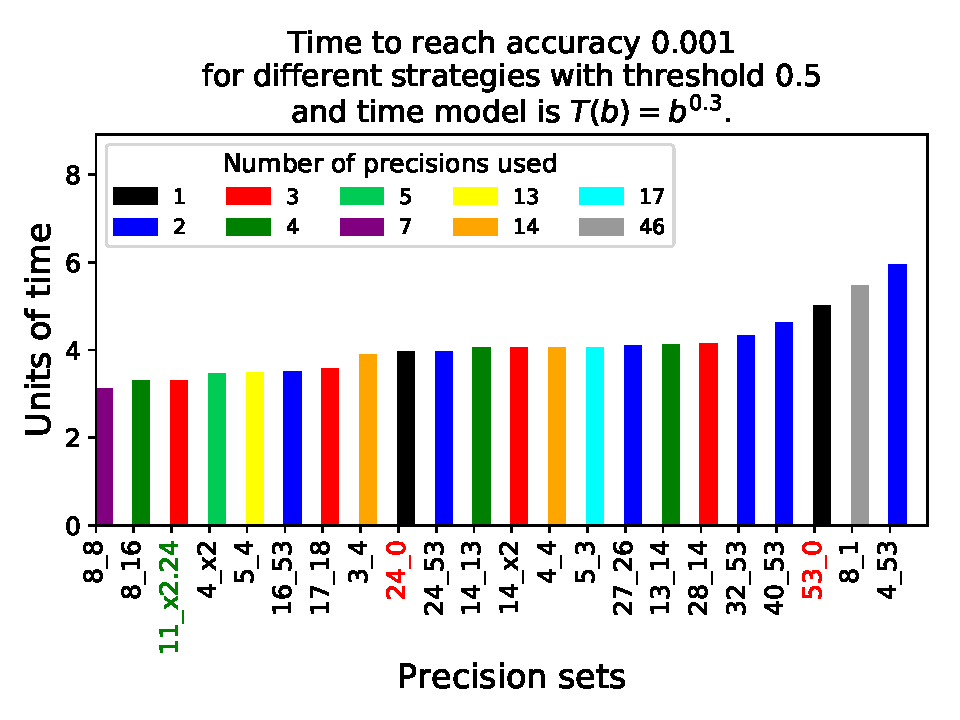
\includegraphics[width=0.33\linewidth]{figs/cost_3_2.pdf}
    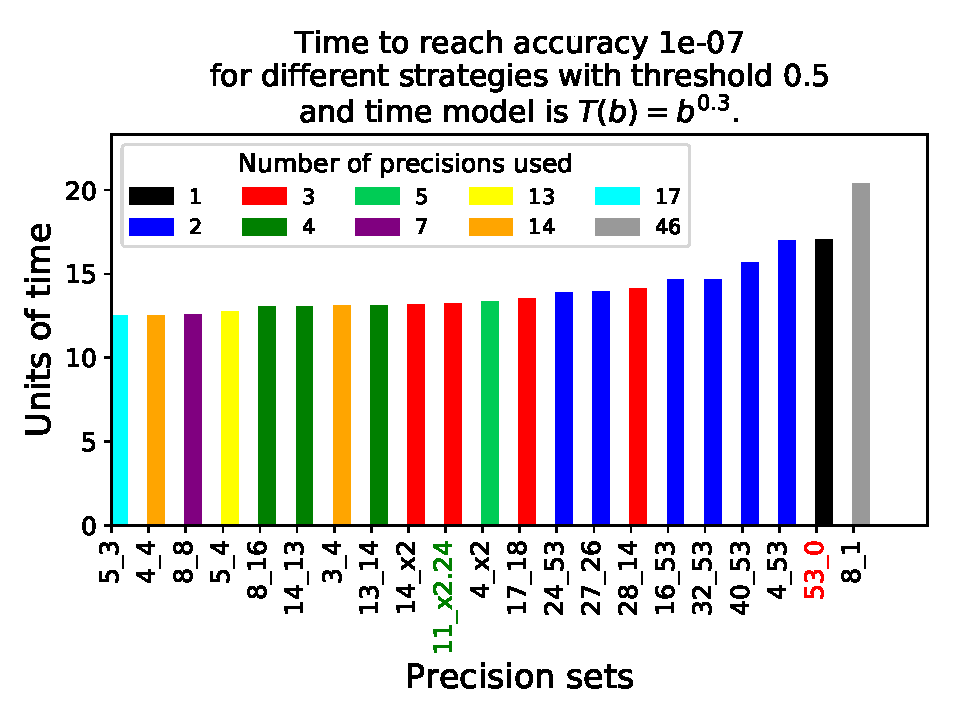
\includegraphics[width=0.33\linewidth]{figs/cost_7_2.pdf}
    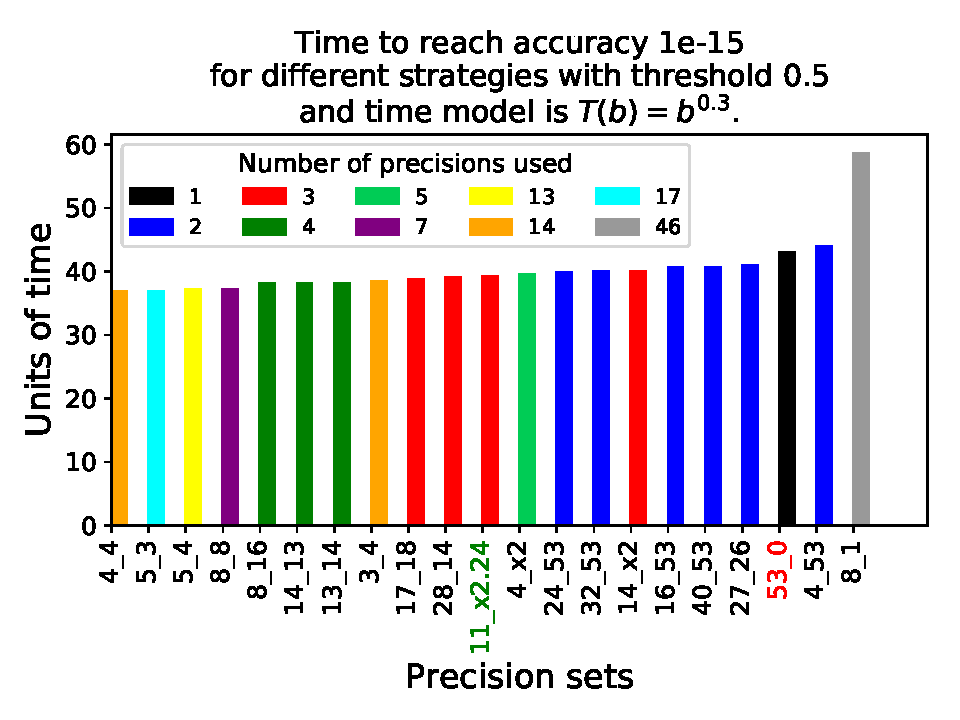
\includegraphics[width=0.33\linewidth]{figs/cost_15_2.pdf}
    \caption{Cost of the MG solver considering several different dynamic
    precision scenarios to reach different error degrees in the output:
    $10^{-3}$ on the left, $10^{-7}$ in the middle and $10^{-15}$ on the
    right. Red labels indicate current performances with either single-precision or double-precision floating-points. Green label indicates the
    performance using a mix of half-, single- and double-precision floating point as available on a GPU.}
    \label{fig.estimation1}
\end{figure*}

To provide numerical values for $a,c$ and most importantly $\alpha$, we measure
the execution times of different scenarios. Each scenario computes 50
iterations on matrices with different sizes, and using either only
single-precision floating point variables or only double-precision floating
point variables. We denote by $x_{b,n}$ the empirical value obtained using $b$
bits and a problem of size $n$ (i.e. the matrix considered will be of size $n^3
\times n^3$ as we consider 3D problems).

%Results are reported in Table~\ref{table.time_measure1}.

\begin{table*}[t]
    \begin{center}
    \resizebox{\textwidth}{!}{
    \begin{tabular}{|c|c|c|c|c|c|c|}
    \hline
    Tolerance & Baseline (DP) & \emph{Up}-cycle (DP) & Adaptive (V-cycle) & Adaptive (\emph{Up}-cycle) & Improvement (DP) & Improvement (SP) \\
    \hline
    \hline
    1e-01 & 1.000 & 1.333 & 0.624 & 0.832 & 16.8\% & -5.5\%\\
    \hline
    1e-02 & 3.000 & 2.000 & 1.872 & 1.664 & 44.5\% & 29.7\%\\
    \hline
    1e-03 & 5.000 & 4.667 & 3.284 & 3.131 & 37.4\% & 20.6\%\\
    \hline
    1e-04 & 8.000 & 7.333 & 5.650 & 5.234 & 34.6\% & 17.0\%\\
    \hline
    1e-05 & 11.000 & 10.0 & 8.015 & 7.336 & 33.3\% & 15.4\% \\
    \hline
    1e-06 & 14.000 & 12.667 & 10.380 & 9.439 & 32.6\% & 14.5\%\\
    \hline
    1e-07 & 17.000 & 15.333 & 13.169 & 11.964 & 29.6\% & -\\
    \hline
    1e-08 & 20.000 & 18.000 & 16.169 & 14.631 & 26.8\% & -\\
    \hline
    1e-09 & 23.000 & 20.667 & 19.169 & 17.298 & 24.8\% & -\\
    \hline
    1e-10 & 26.000 & 24.000 & 22.169 & 20.631 & 20.7\% & -\\
    \hline
    1e-11 & 29.000 & 26.667 & 25.169 & 23.298 & 19.7\%& -\\
    \hline
    1e-12 & 32.000 & 29.333 & 28.169 & 25.964 & 18.9\% & -\\
    \hline
    1e-13 & 35.000 & 32.000 & 31.169 & 28.631 & 18.2\% & -\\
    \hline
    1e-14 & 38.000 & 34.667 & 34.169 & 31.298 & 17.6\% & -\\
    \hline
    1e-15 & 43.000 & 39.333 & 39.169 & 35.964 & 16.4\% & -\\
    \hline
    \end{tabular}
    }
    \end{center}
    \caption{All estimated times for \textsc{Unstructured-Anisotropy}, size 40,
    hybrid relaxation method, on a single processor, with $\alpha = 0.3$. The
    column `Improvement (DP)' corresponds to the improvement between the
    adaptive algorithm using a \emph{Up}-cycle (column 5) compared to the
    original V-cycle with fixed double-precision (column 2). The column
    `Improvement (SP)' corresponds to the improvement between the adaptive
    algorithm using a \emph{Up}-cycle (column 5) compared to the original
    V-cycle with fixed single-precision.}
    \label{table.results1}
\end{table*}

Then, using Python's lmfit package, we interpolate the data to find good values
for $a,c$ and $\alpha$. We are able to estimate different values of $\alpha$,
all between 0.20 and 0.32, using 3 different applications, 2 types of cycles
(the classic V-cycle and the \emph{Up} strategy) and 2 types of relaxation
methods (weighted Jacobi and an hybrid method).  Each data-fitting was done on
either 30 or 40 points.  With these values of $\alpha$, we can estimate the
cost of our algorithm in units of time by $\left(\frac{b}{53}\right)^\alpha$
for a cycle (1 unit = 1 V-cycle at double-precision) with $b$ the number of
significant bits (i.e. the number of bits in the mantissa plus one, as one bit
is always assumed in standard floating point representation). Then using the
MPFR library we can create different scenarios that set the number of bits used
at each cycle in a different way. We define all these scenarios by the first
precision ($b$ in the mantissa) used and how to update it ($delta$ bits added
in the mantissa when the threshold is reached for a given precision).
Strategies are denoted as $b\_delta$. This can be either an addition or a
multiplication. In particular, we provide a scenario where the available
mantissa precisions are 11, 24 and 53 (represented by a starting mantissa
precision of 11 and a multiplicator of 2.24, in green on Figure~\ref{fig.estimation1}). This corresponds to the case
where the computation starts in half-precision, then switches to
single-precision and finally to double-precision. This scenario is particularly
relevant because those precisions are already available in architectures such
as the recent Volta GPUs which integrates Tensor cores in half-precision.

%\begin{figure}
   % 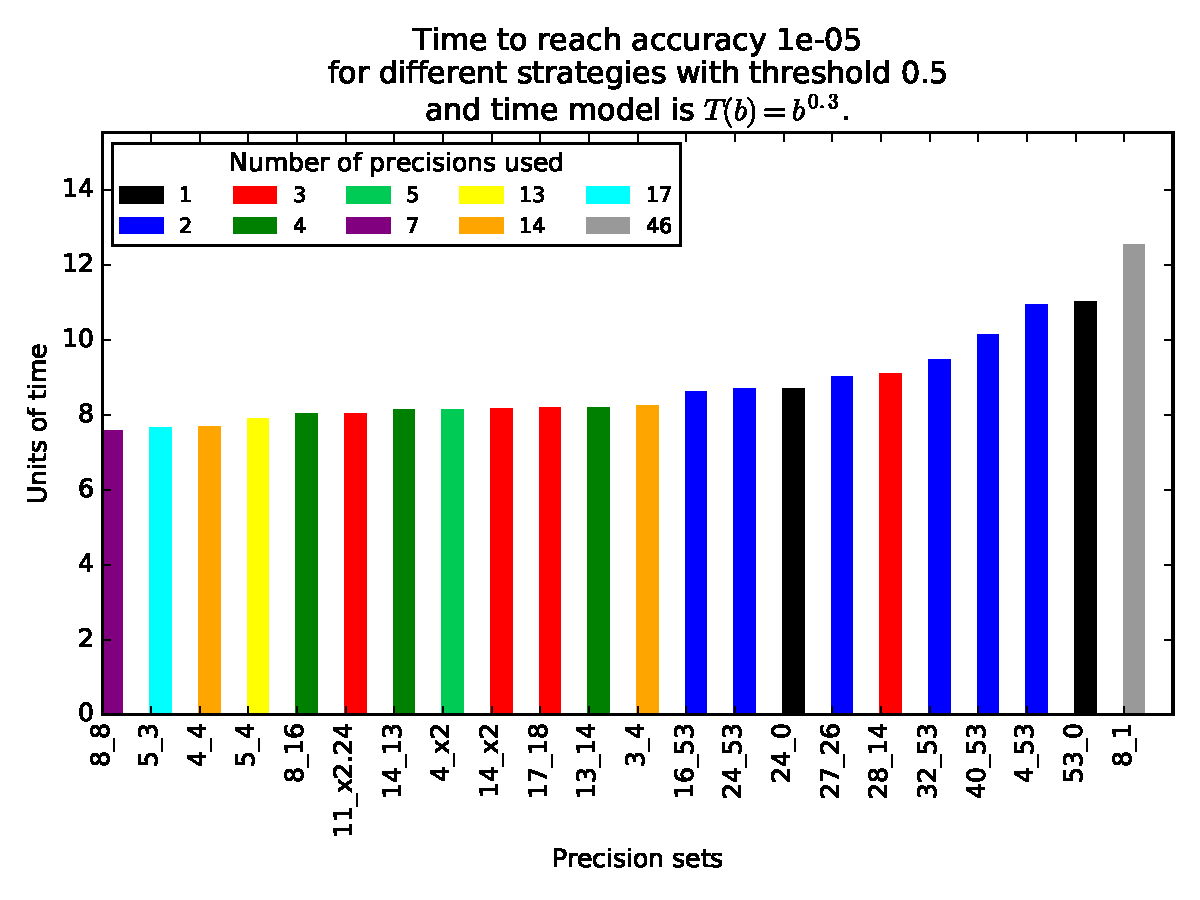
\includegraphics[width=\linewidth]{figs/cost_5.pdf}
   % \caption{}
   % \label{fig.estimation2}
   %\end{figure}
   %\begin{figure}
   % 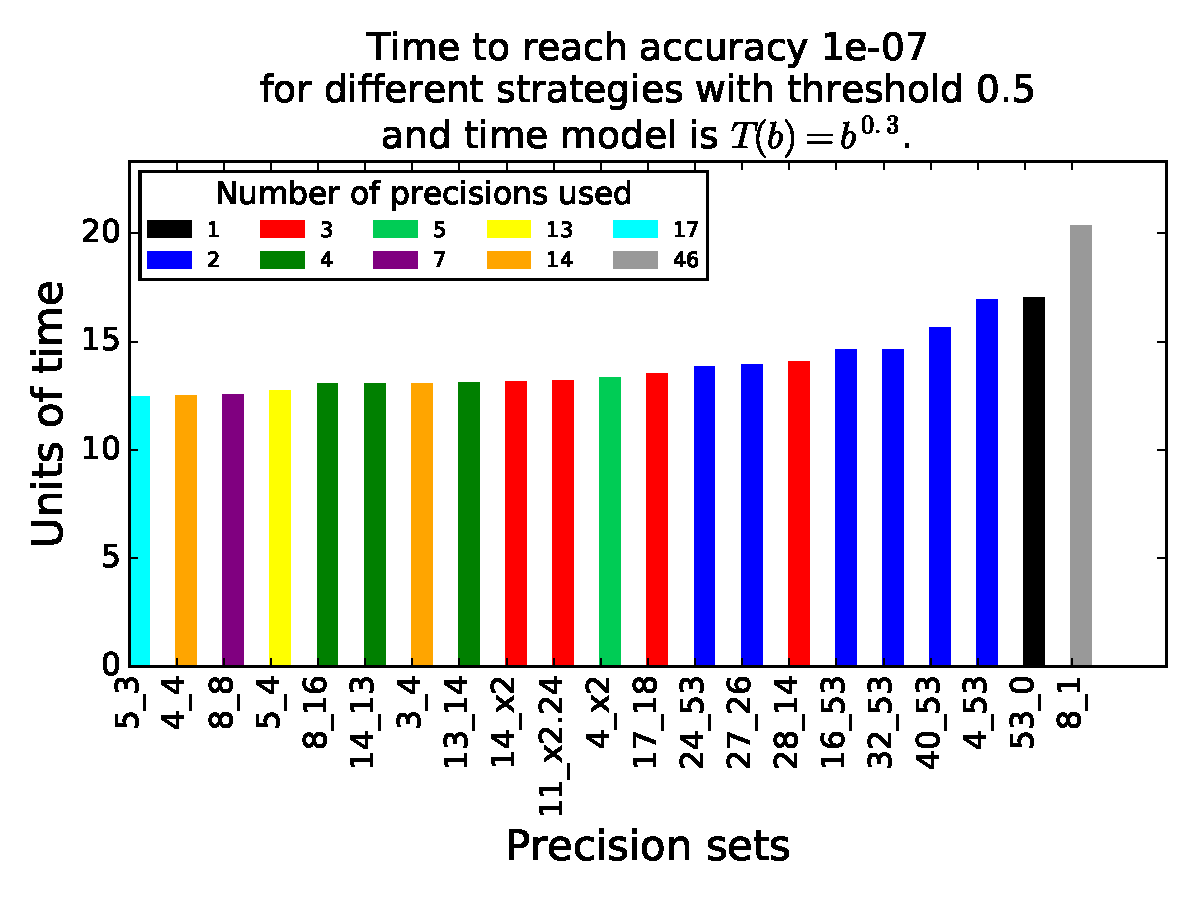
\includegraphics[width=\linewidth]{figs/cost_7.pdf}
   % \caption{}
   % \label{fig.estimation3}
   %\end{figure}
   %\begin{figure}
   % 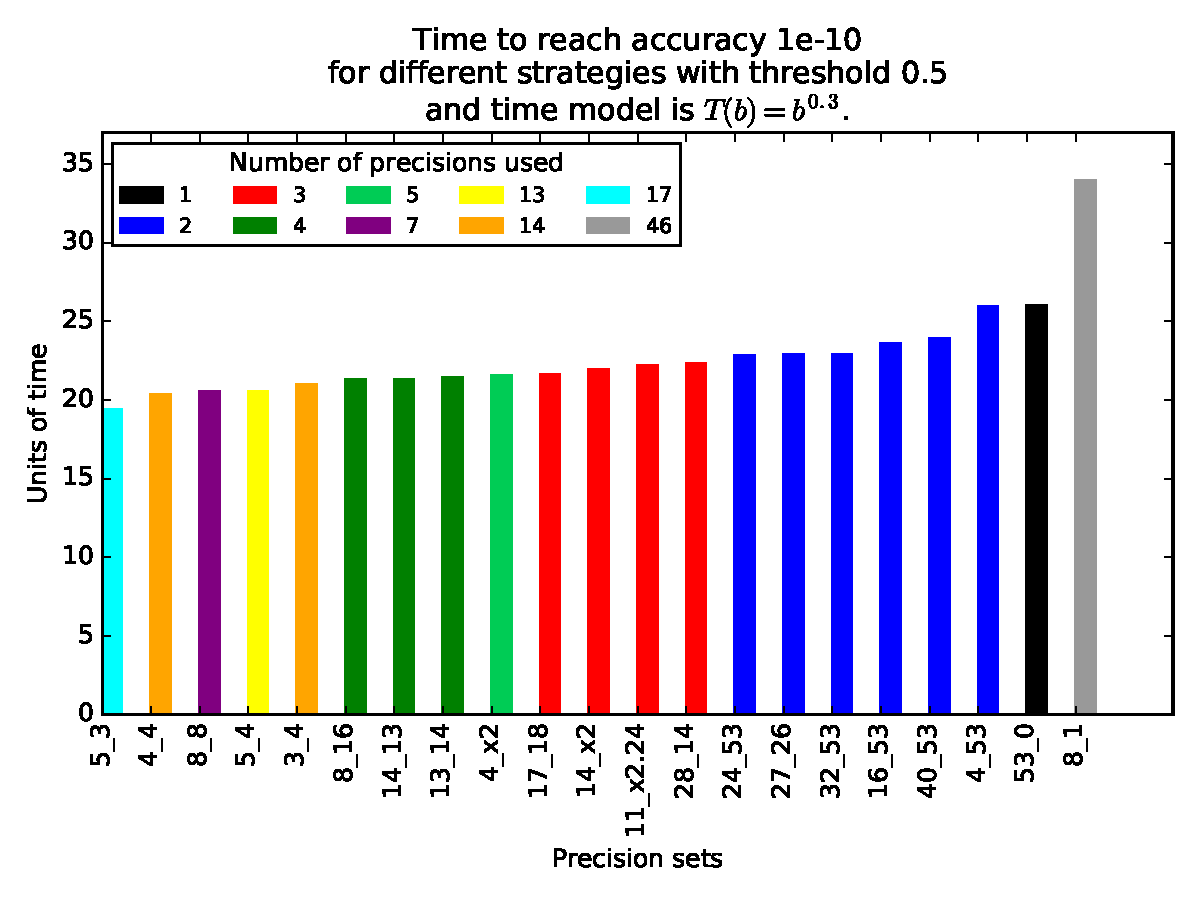
\includegraphics[width=\linewidth]{figs/cost_10.pdf}
   % \caption{}
   % \label{fig.estimation4}
   %\end{figure}
   %\begin{figure}
   % 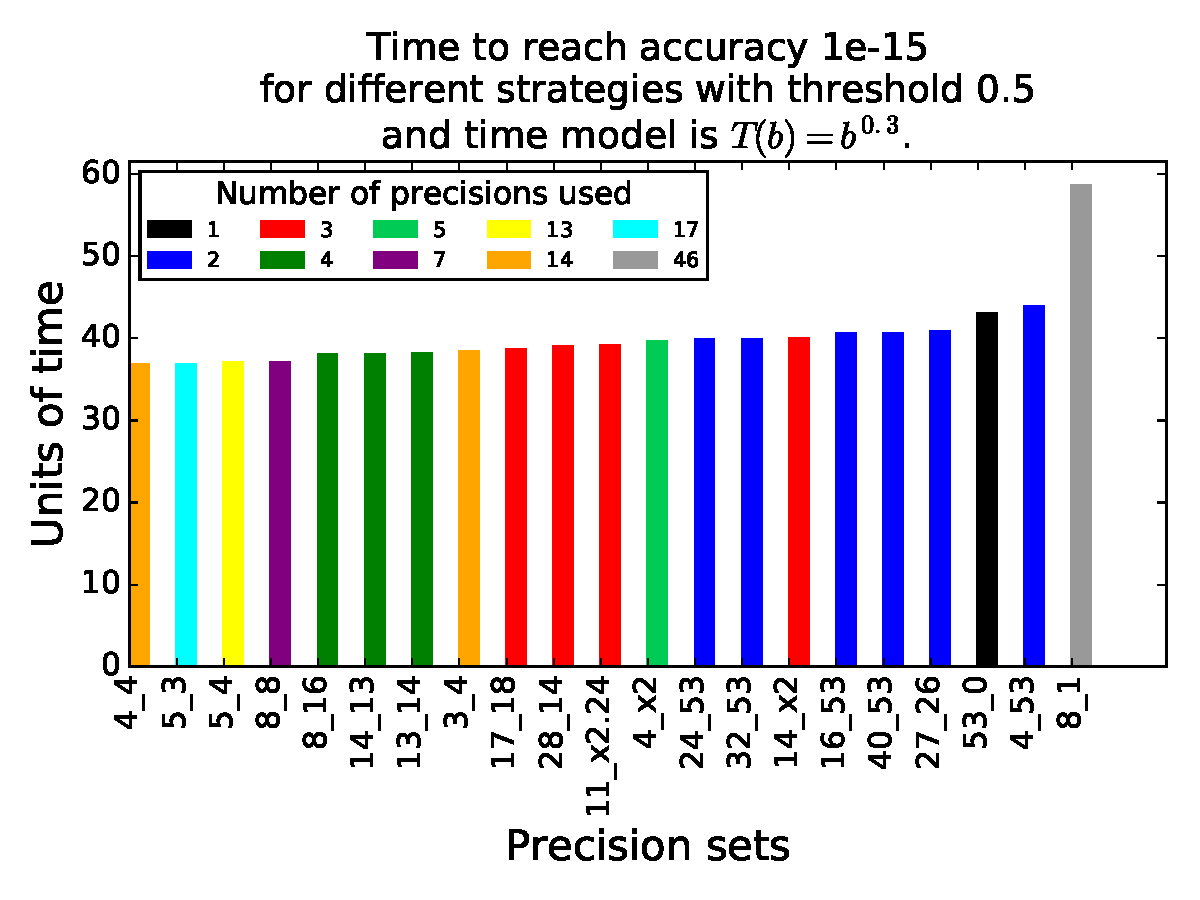
\includegraphics[width=\linewidth]{figs/cost_15.pdf}
   % \caption{}
   % \label{fig.estimation5}
   %\end{figure}

Figure~\ref{fig.estimation1} represents the cost of the MG solver, for these
different scenarios, to reach different accuracy degrees in the output
($10^{-3}$ on the left, $10^{-7}$ in the middle and $10^{-15}$ on the right)
using a value for the $\alpha$ parameter of $0.3$. We can see that the strategy
that increases by only 1 the number of mantissa bits (labelled \texttt{8\_1})
takes more time than the original algorithm (labelled \texttt{53\_0}) for the 3
different accuracies presented. This is because, in the previous experiments we
saw there is usually the same number of cycles in all our strategies (see
Figure~\ref{fig.prec_incr}). Here, the convergence rate is limited by slowly
increasing number of precision bits: by adding one bit we can reduce by at most
2 the error on the residual norm, while the original algorithm can reduce the
error by more than that in one cycle when it is not limited by the bit-width of
the variables.

If we focus on a case starting with half precision, then going to single and
finally to double precision (labelled \texttt{11\_x2.24}), we can see that,
compared to the original algorithm (which uses only double-precision), we
improve by 35\% the time to reach accuracy $10^{-3}$ (see
Figure~\ref{fig.estimation1}). If one adapts the algorithm to use only
single-precision variables (labelled \texttt{24\_0}) as it would be sufficient
to reach this accuracy, we would still reduce the time by 17\% (still
Figure~\ref{fig.estimation1}). When higher accuracy is needed in the final
result, the performance improvement by adapting precisions is still quite
important, around 10\% faster than using double precision (See $10^{-15}$ on
Figure~\ref{fig.estimation1}).


\subsection{Putting it all Together}

Finally, we want to see how changing the precisions during the algorithm also
improves the execution time when we use the \emph{Up} strategy, defined in
section~\ref{sec.assymetric}, compared to using the original algorithm (single
or double precision). The table~\ref{table.results1} presents the different
estimated times (in time units where 1 time unit is a V-cycle at double
precision) for all 4 different algorithms: V-cycle (double precision),
\emph{Up}-cycle (double precision), V-cycle (adaptive precisions 11-24-53),
\emph{Up}-cycle (adaptive precisions 11-24-53) for Problem 1, using a hybrid
relaxation method.  We also present the improvement of the best method (i.e.
\emph{Up}-cycle with different precisions) compared to the original algorithm
(in double-precision and in single-precision when possible).

The main result is that even to reach the maximum precision, we improve the
execution time by more than 15\%. When it comes to smaller precisions, this
improvement can be as high as 30\% compared to a single-precision algorithm and
it even goes up to 45\% compared to the original double-precision version. We
want to highlight that these results for the adaptive algorithm use 3 different
mantissa precisions (11,24,53) (i.e., half, single, double) already available
in current hardware. More aggressive adaptations (e.g., \texttt{4\_4}) could be
potentially implemented in architectures such as FPGAs leading to even faster
executions, as shown in Figure~\ref{fig.estimation1}.




%% Section VI
\section{Related Work}
\label{sec:related}

   Some approximate computing techniques at hardware level exist and could be applied in addition to our ideas. They include fast but slightly incorrect adders~\cite{Gupta:2011}, or voltage-scaling (in SRAM, reducing
   the voltage by 80\% increases the probability of an unexpected bit flip by around $10^{-5}$~\cite{Sampson:2011})
   if we are more interested in reducing the energy consumption instead of the execution time.\\
   Concerning multi-grid algorithms, the opposite of our \emph{Up} strategy has been considered in~\cite{JAMESON}: they do some actual computation when going down in the grid and then simply interpolate to retrieve the solution on the finest grid. The reason for that is that they
   address a specific problem where some perturbations need to be damped quite efficiently, which is why as soon as they perform some computation on the fine grid they need to use coarse grids even if interpolating directly introduces some errors.
   Dynamically changing the bit-width of some variables has been done in~\cite{Park:2010} but it is there applied on some part of the data as they are not involved in the same way in the algorithm,
   which is not the case in a multi-grid solver (all the evaluation points on the grid represent the continuous solution).




%% Section VII
\section{Conclusion}
\label{sec:conclusions}

This paper improves the original MG algorithm by two different ways: 
The first one is to remove some relaxation steps in a V-cycle, which leads to faster cycles although requires more of them to converge.
Overall, this solution achieves up to 30\% improvement although its performance enhancements vary a lot depending on the workload,
The second way to improve the algorithm is to adapt the precisions of the floating point depending on MG's precision requirements,
We use low precisions levels during the very first MG's cycles and we increase them as the execution progresses. 
Repeating this operation until reaching the maximum available accuracy available leads to significant speedups.
We estimate the benefits of these two approaches combined on different scenarios. 
When combining half-, single- and double-precisions, we can reduce by 16.4\% and 14.5\% the execution time using double- or single-precision, respectively, during the whole execution. 

In the future we plan to explore additional ideas to reduce the execution time even more like changing the precision used in different levels of a cycle. 
%However, we think that it is not
%   useful because (1) using a greater precision in the coarse levels than in the fine levels is useless as all the computations would eventually be truncated and (2) using a smaller
%   precision in the coarse levels than in the fine levels would not affect by much the execution time as, according to the measurements done, only the first 2 or 3 levels represent more than 95\% of the relaxation cost of a cycle.
Also, we plan to estimate the impact of our techniques on the energy consumption by obtaining some measurements on real machines.
Evaluating the energy consumption using different values of the $\alpha$ parameter is also in our immediate future plans.


%% References
\bibliography{biblio}
\bibliographystyle{plain}

\end{document}
